\documentclass[10pt]{beamer}
\usepackage{hyperref}
\usepackage{xcolor}
\usepackage[export]{adjustbox} %used to align the images
\usepackage{tabularx}
\usepackage{lmodern,textcomp}
\usepackage[font=tiny]{caption}
\usepackage{color,soul}
\usepackage{booktabs}

%\usetheme{Berlin}
\usetheme{Madrid}
\title{Deliverable 2: Applicazione di tecniche di ML su progetti open source}
%\subtitle{}
\author{Pierciro Caliandro}
\institute{Università degli studi di Roma Tor Vergata}

\definecolor{blue}{rgb}{0.0, 0.0, 1.0}
\definecolor{calpolypomonagreen}{rgb}{0.12, 0.3, 0.17}

\setbeamercolor{palette primary}{bg=calpolypomonagreen, fg=white}
%\setbeamercolor{palette secondary}{bg=calpolypomonagreen, fg=white}

\usecolortheme[named=blue]{structure}


\begin{document}
\footnotesize
\begin{frame}
\titlepage
\end{frame}

\begin{frame}{Indice}
\tableofcontents
\end{frame}

\begin{frame}
\section{Introduzione}
\frametitle{Introduzione}
\begin{itemize}
\item Lo scopo della presentazione è quello di mostrare i risultati a seguito dell'applicazione di tecniche di sampling, classificazioni
sensibili al costo, e feature selection su modelli di ML. In particolare, ci si concentra su come tali tecniche impattano sulle metriche di accuratezza per i seguenti classificatori:
\begin{itemize}
\item[-] NaiveBayes
\item[-] RandomForest
\item[-] Ibk
\end{itemize}
\item I dati forniti ai classificatori per il training ed il testing sono stati raccolti da due progetti open source della Apache Software Foundation:
\begin{itemize}
\item[-] Apache BookKeeper
\item[-] Apache ZooKeeper
\end{itemize}
\item Le analisi partono dai risultati ottenuti, per tutti i classificatori, senza l'applicazione di alcuna tecnica per poi vedere con quali tecniche e per quali classificatori si ottengono risultati migliori
\end{itemize}
\end{frame}

\begin{frame}
\section{Derivazione dei dataset}
\frametitle{Derivazione dei dataset}
\begin{itemize}
\item Come prima cosa, per entrambi i progetti, è stata utlizzata la rest API di Jira per poter ottenere tutti i Ticket di tipo bug relativi ad entrambi i progetti
\item Dopo aver ordinati i ticket in base alle loro date di risoluzione, sono stati trovati ed ordinati i corrispettivi commit andando a consultare il log ottenibile da git, per fare ciò si è utilizzato il tool \href{https://wiki.eclipse.org/JGit/User_Guide}{JGit}
\item A questo punto, scorrendo le varie release, sono state calcolate le 9 metriche scelte per entrambi i progetti, andando poi a riempire un file csv per ogni singolo progetto. Per ciascun progetto, vengono riportati solo i dati relativi alla prima metà del totale delle release
\end{itemize}
\end{frame}

\begin{frame}
\subsection{Struttura del dataset}
\frametitle{Struttura del dataset}
\begin{itemize}
\item La struttura di entrambi i dataset è la seguente:
\begin{figure}
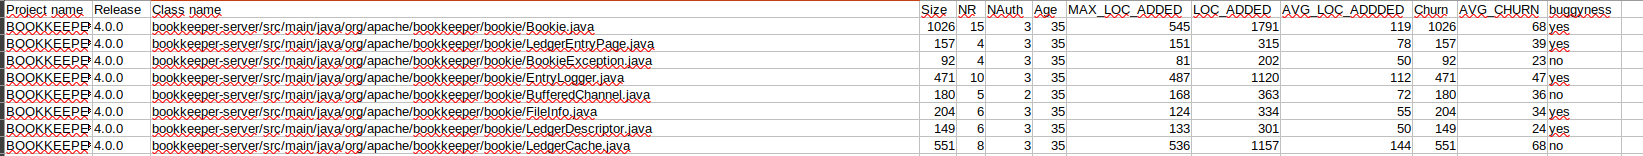
\includegraphics[scale=0.19]{images/csv-header}
\caption{Header per i file csv}
\end{figure}
\item In entrambi i dataset sono stati riportati 9 metriche, relative alla singola classe, usate poi dai classificatori per stimare se una classe presentasse un bug in una determinata release:
\begin{minipage}[t]{0.4\textwidth}
\begin{itemize}
\item Size: numero di LOC 
\item NR: Numero di revisioni
\item NAuth: Numero di autori della classe
\item Age: 'età', in settimane
\item MAX\_LOC\_ADDED: massimo numero di LOC aggiunte in una release
\end{itemize}
\end{minipage}%
\begin{minipage}[t]{0.5\textwidth}
\begin{itemize}
\item LOC\_ADDED: LOC aggiunte in una release
\item AVG\_LOC\_ADDED: media di LOC aggiunte in una release
\item Churn: differenza fra LOC aggiunte e rimosse
\item AVG\_Churn: media della differenza fra LOC aggiunte e rimosse
\end{itemize}
\end{minipage}%
\item L'ultimo  attributo del dataset è la buggyness nella release corrente,  calcolata usando le Affected Version quando disponibili dai ticket di Jira, o altrimenti applicando il metodo proportion per stimare le affected version
\end{itemize} 
\end{frame}

\begin{frame}
\section{Tecnica di classificazione}
\frametitle{Tecnica di classificazione}
\begin{itemize}
\item La tecnica di calssificazione utilizzata è Walk Forward
\item Il training set è stato incrementato di volta in volta, andando ad aggiungere sempre i dati relativi alla successiva release
\item Per il testing set si usa sempre la prima release non ancora inclusa nel training set
\item Ad esempio, per la prima run si avrà il training set contenente la release 1 ed il testing set formato dalla release 2. Nella run successiva il training set sarà costituito dalle release 1 e 2, mentre il testing set dalla release 3
\item Per la classificazione, è stato usato il tool weka, sfruttando sia la API che la versione stand alone.
\item I valori riportati nei due dataset sono stati calcolati dall'API, e confrontati con quanto veniva riportato dall'esecuzione sugli stessi dati con la versione stand alone
\end{itemize} 
\end{frame}

\begin{frame}
\section{Tecniche utilizzate}
\frametitle{Tecniche utilizzate}
\begin{itemize}
\item Per cercare di migliorare i valori ottenuti dalla prima analisi, sono state applicate alcune tecniche:
\begin{itemize}
\item Feature Selection, utilizzando Best First come tecnica
\item Sampling, utilizzando 
\begin{itemize}
\item under-sampling: vengono diminuite le istanze della classe maggioritaria fino a pareggiare quelle della classe minoritaria
\item over-samplig: vengono aumentate le istanze della classe minoritaria fino a pareggiare quelle della classe maggioritaria
\item SMOTE: vengono create istanze aggiuntive per la classe minoritaria in maniera "sintetica"
\end{itemize}
\item Cost sensitive valuation, usando:
\begin{itemize}
\item sensitive threshold, viene aggiustato il valore della threshold
\item sensitive learning, le classi vengono replicate in base al peso, quindi è come se venissero ripesate
\end{itemize}
In entrambe i casi, la matrice dei costi prevede un costo 10 volte maggiore per un falso negativo rispetto a quello per un falso positivo
\end{itemize}
\end{itemize} 
\end{frame}

\begin{frame}
\section{Metriche analizzate}
\frametitle{Metriche analizzate}
\begin{itemize}
\item Sono stati considerati ed analizzati i valori per le seguenti metriche di performance:
\begin{itemize}
\item AUC: Area Under The Curve, area sottesa alla ROC che da una misura di quanto il classificatore è in grado di predirre correttamente una istanza positiva scelta casualmente con un valore più alto di uno per una istanza negativa presa casualmente
\item Recall: definita come $\frac{TP}{TP+FN}$, che fornisce una misura relativamente a quanti valori positivi sono stati classificati su quanti effettivamente ce ne erano
\item Precision: definita come$\frac{TP}{TP+FP}$, da una misura dell'errore che si commette nello stimare un positivo, quindi aiuta nel poter capire quanto è attendibile il valore di Recall.
\item Kappa: metrica che definisce quanto il classificatore è meglio rispetto ad un classificatore dummy, ovvero puramente randomico
\end{itemize}
\end{itemize} 
\end{frame}

\begin{frame}
\subsection{Analisi dei valori}
\frametitle{Analisi dei valori}
\begin{itemize}
\item Per alcune metriche, l'analisi dei valori è stata guidata dal confronto con i valori che si avrebbero se si usasse un classificatore "dummy", ovvero random
\item Per la AUC, avere un valore pari a 0.5 vuol dire che il classificatore si comporta come uno random, mentre averlo minore di 0.5 indica un comportamento peggiore
\item La metrica Kappa è un indice di quanto il classificatore va meglio rispetto ad uno random: valori pari a 0 indicano un comportamento del classificatore analogo a quello di uno random, mentre valori minori di 0 ne indicano un comportamento peggiore
\item Precision e Recall vengono analizzate insieme, in quanto la Precision da una indicazione di quanto i valori ottenuti per la Recall siano "affidabili"
\end{itemize} 
\end{frame}

\begin{frame}
\section{Analisi della AUC per BookKeeper}
\frametitle{Analisi della AUC per BookKeeper}
\begin{itemize}
\item Dall'analisi dei valori per la AUC dei tre classificatori, considerando il progetto BookKeeper, è stato estrapolato il seguente box plot:
\begin{figure}
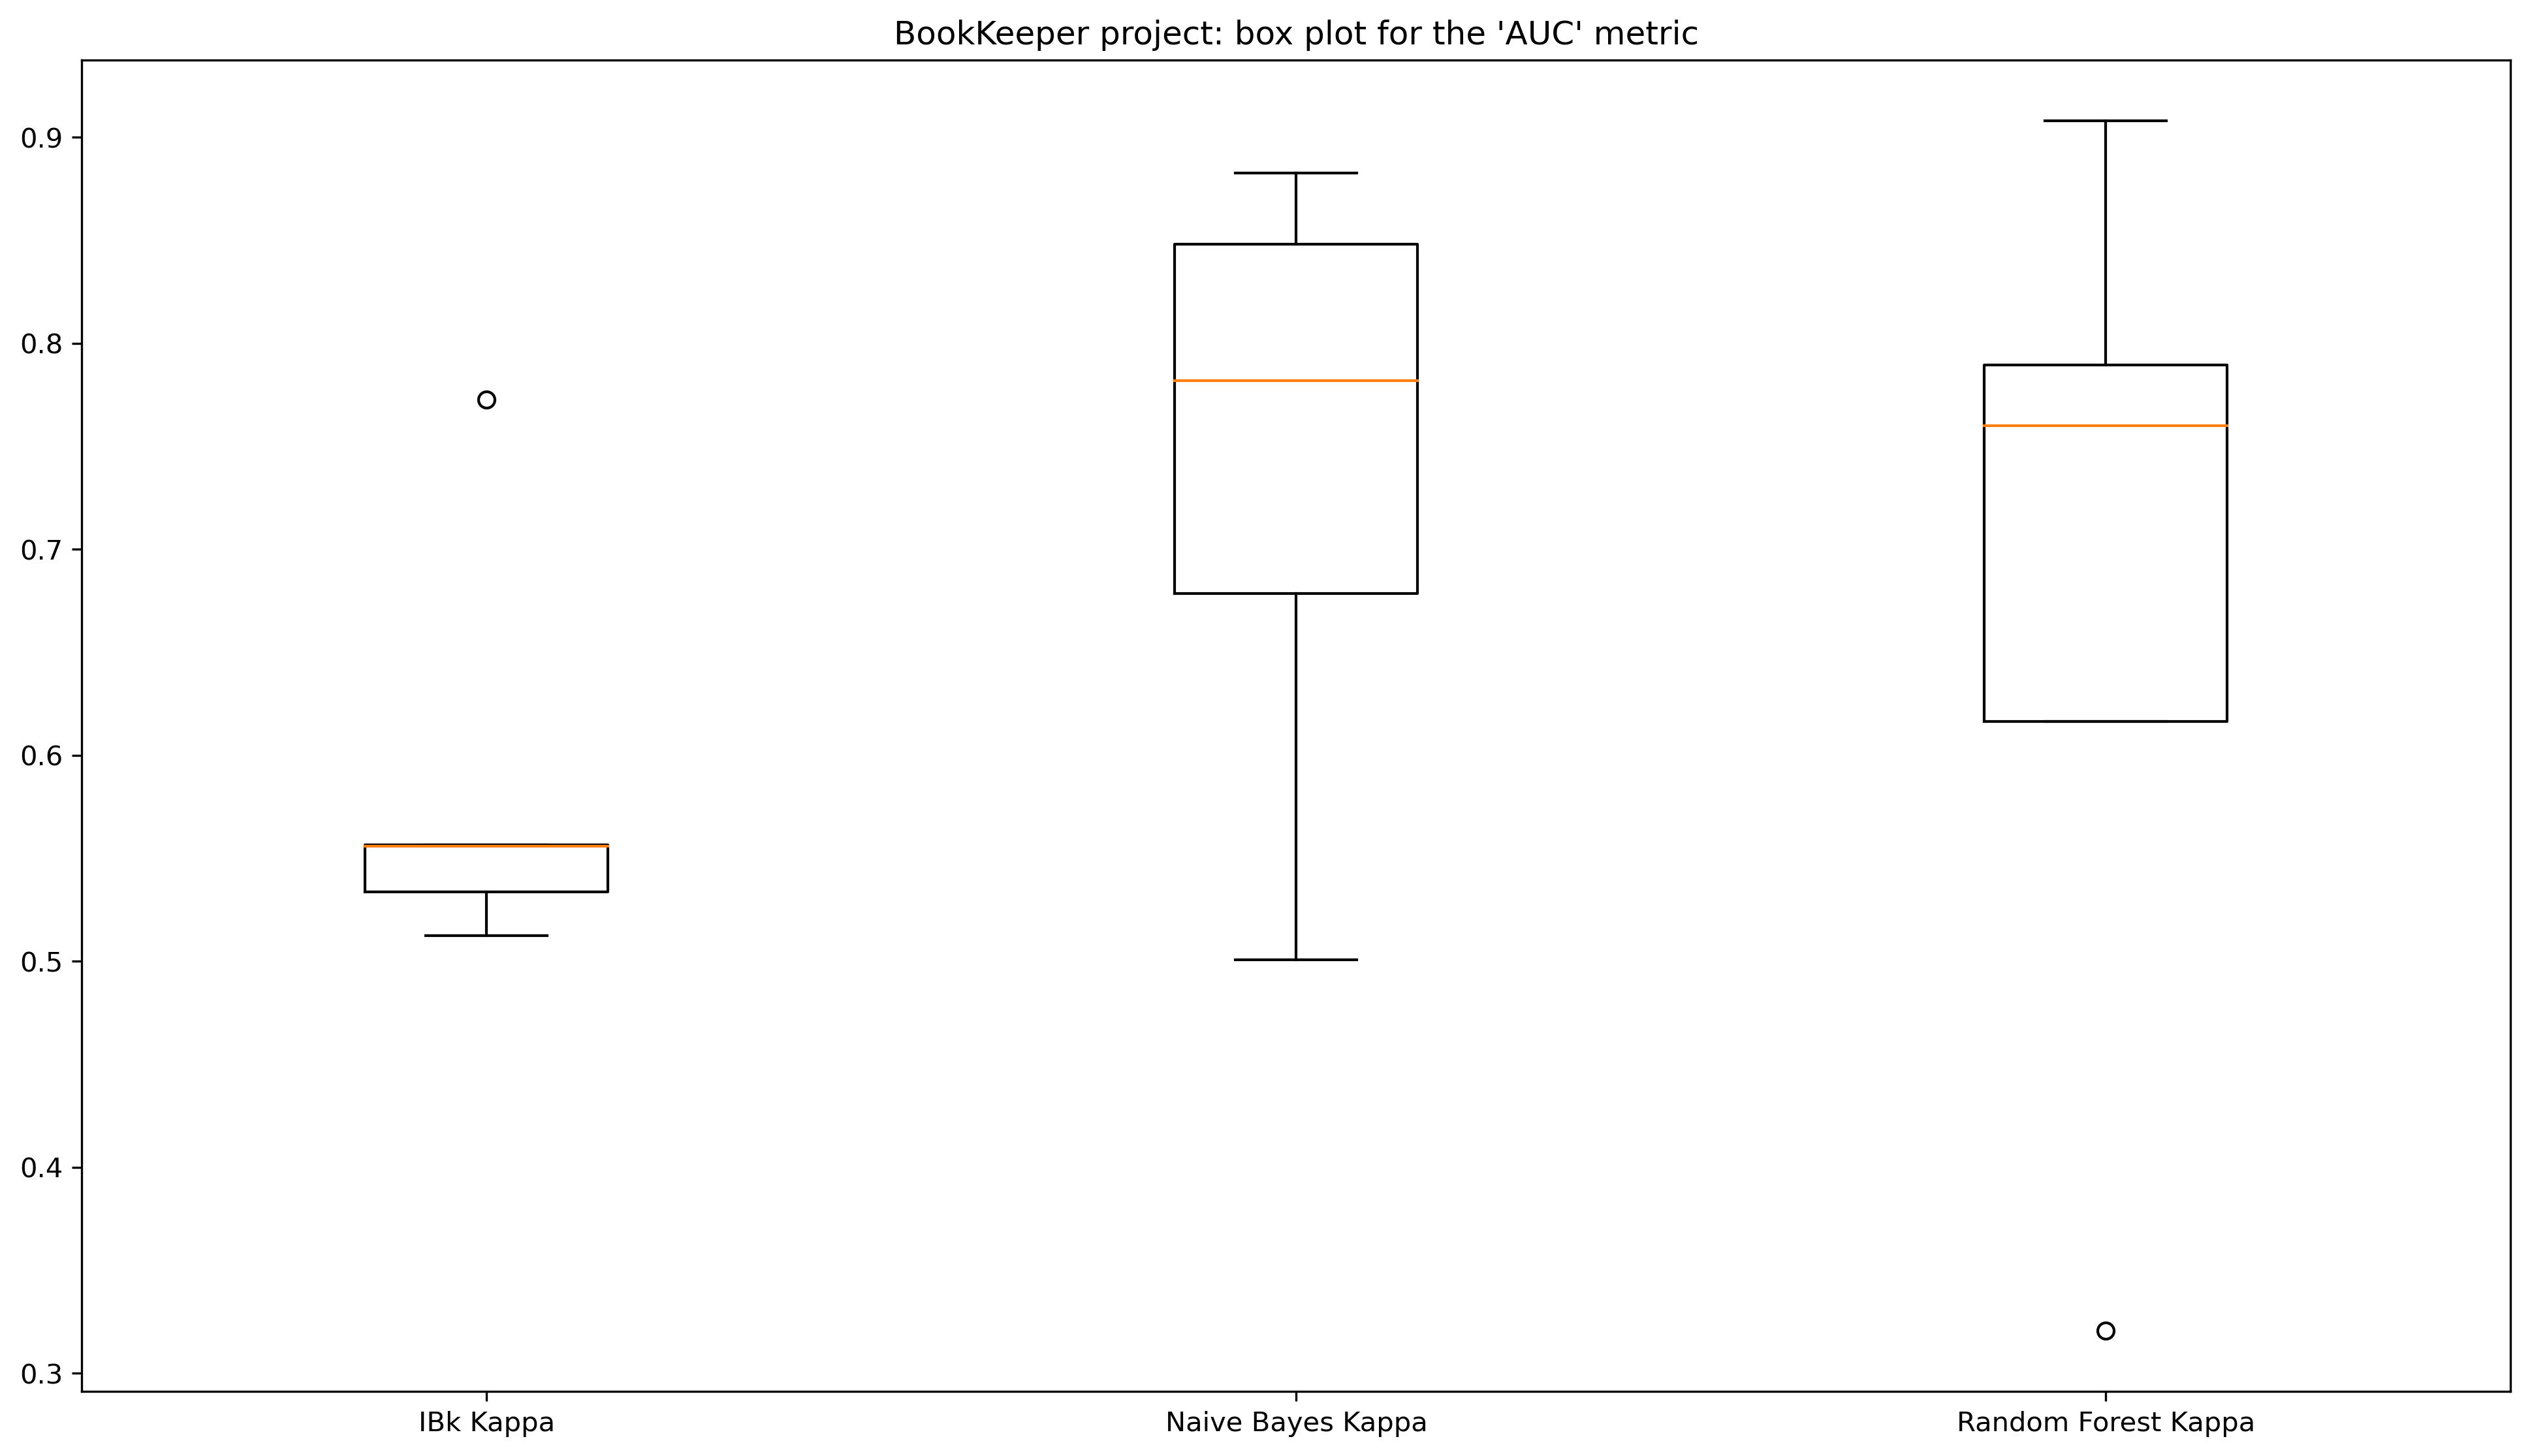
\includegraphics[scale=0.25]{images/auc_base_bk}
\end{figure}
\item IBk presenta un una distribuzione della AUC con valori migliori di quelli di un classificatore random, anche se di poco, con un outlier intorno al valore 0.77
\item Anche Random Forest ha una distribuzione dei valori migliore di quella di un classificatore random, pur presentando un outliers nel punto 0.32
\item Naive Bayes risulta il classificatore con la migliore distribuzione per la metrica AUC
\end{itemize}
\end{frame}

\begin{frame}
\subsection{Analisi della AUC per BookKeeper - miglioramento dei valori}
\frametitle{Analisi della AUC per BookKeeper - miglioramento dei valori}
\begin{itemize}
\item L'analisi successiva dei valori era volta a capire quale tecnica migliorasse il valore per la metrica di AUC per i singoli classificatori
\item Da una prima analisi, risulta che cambiare il valore della metrica peggiora sempre quando viene utilizzato un classificatore cost sensitive
\item Fra tutti, il classificatore su cui ci si è concentrati per l'aumento della metrica è IBk, che mostra i valori peggiori
\item Risulta che l'applicazione di over-sampling e di feature selection migliorano di molto i valori per la metrica IBk, con anche un leggero miglioramento per i valori di Random Forest
\begin{figure}
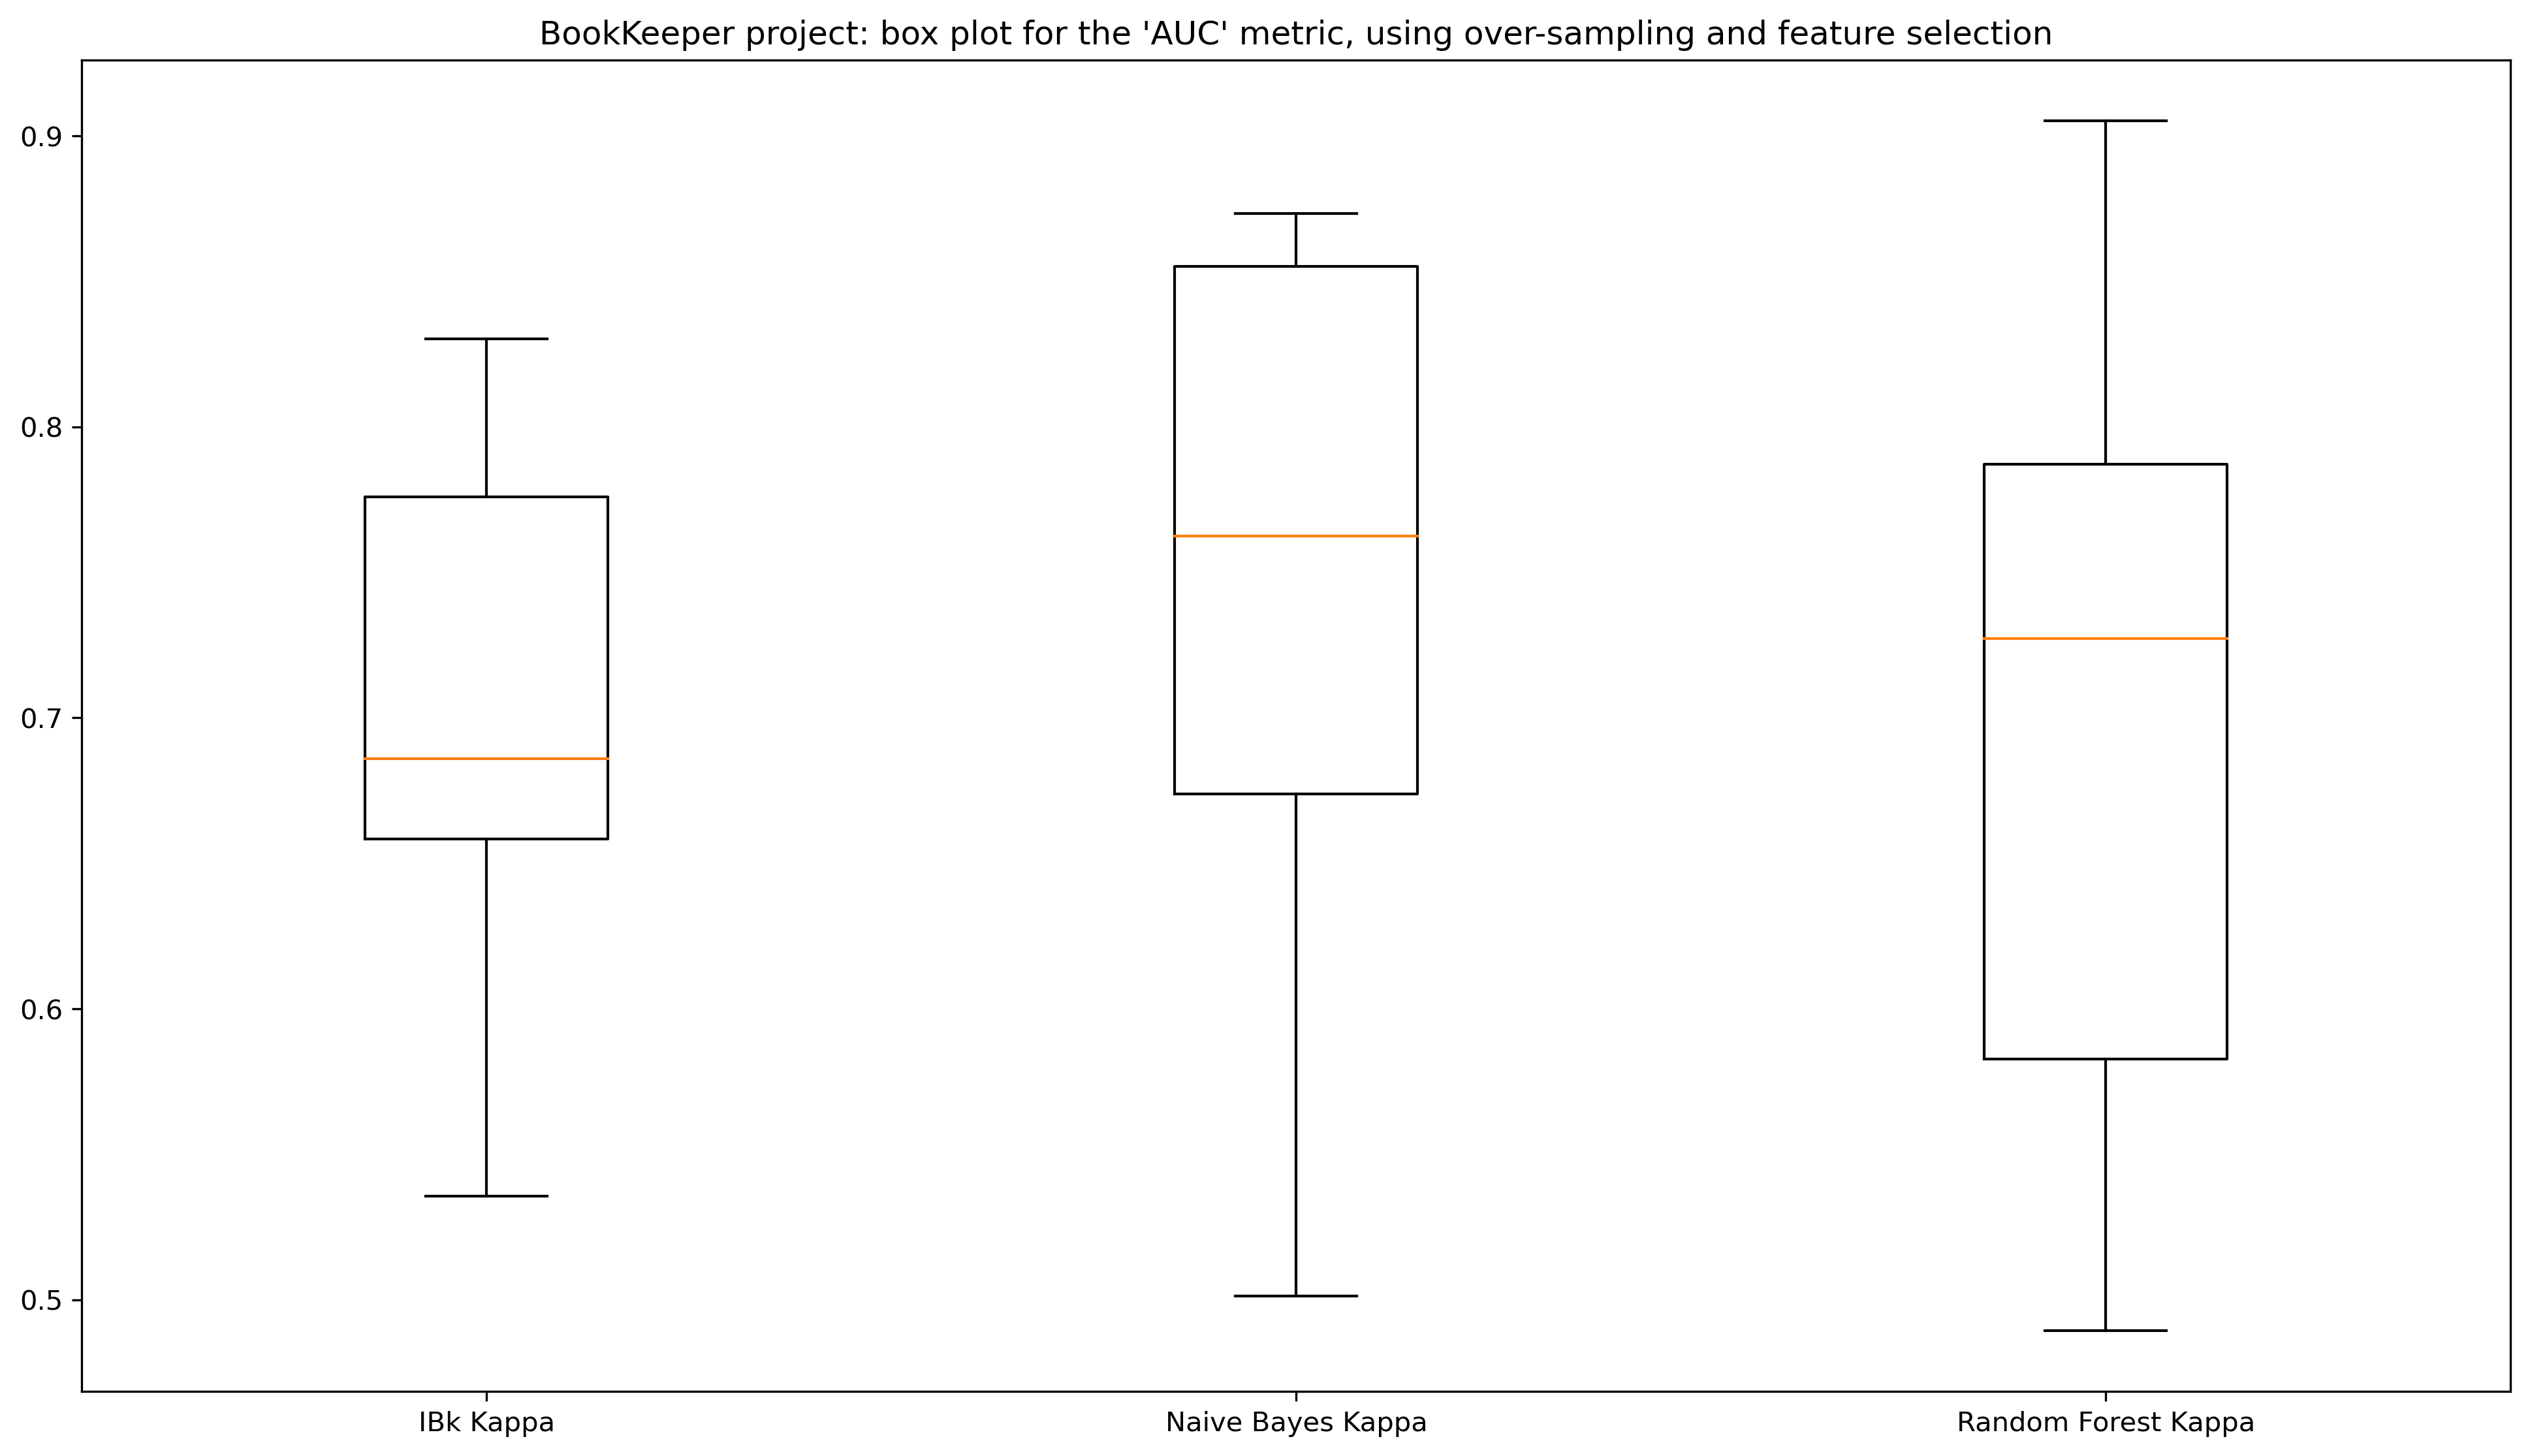
\includegraphics[scale=0.23]{images/auc_bett}
\end{figure}
\end{itemize}
\end{frame}

\begin{frame}
\section{Analisi della AUC per ZooKeeper}
\frametitle{Analisi della AUC per ZooKeeper}
\begin{itemize}
\item Per determinate run, alcuni dei classificatori presentavano NaN come valore della metrica, quindi tali valori sono stati scartati
\item La prima analisi per la AUC sul progetto ZooKeeper fornisce i seguenti risultati:
\begin{figure}
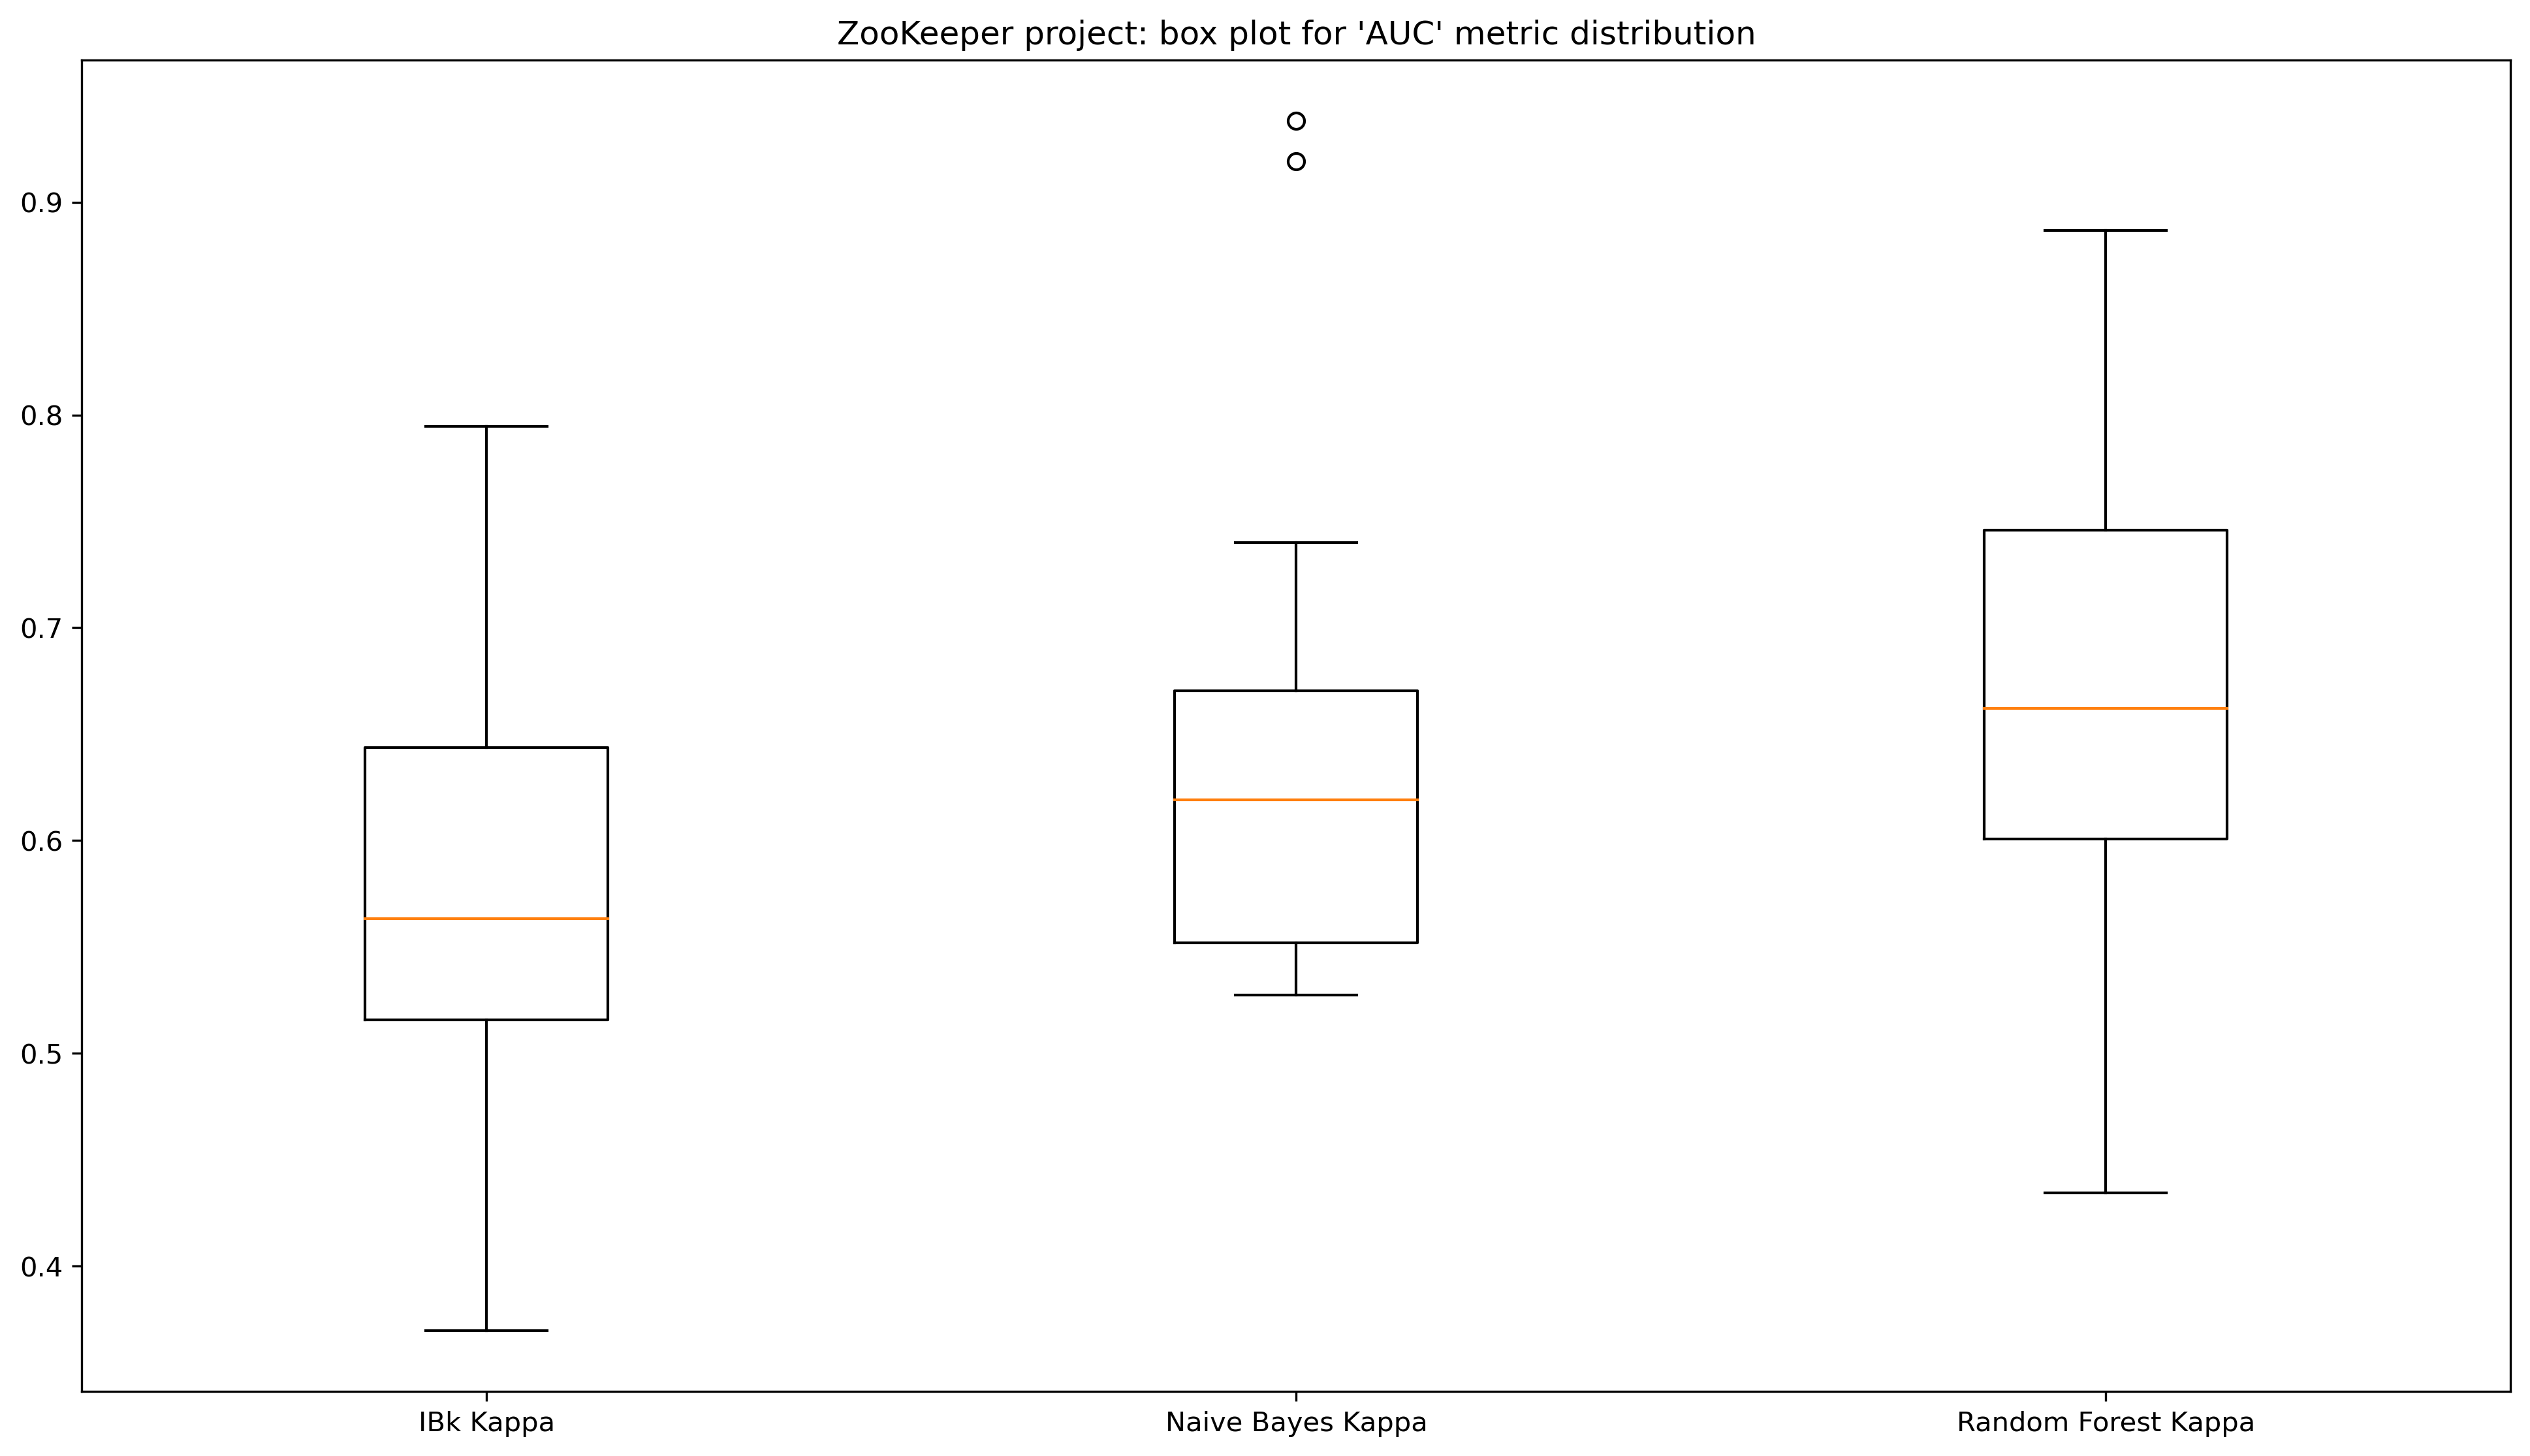
\includegraphics[scale=0.25]{images/auc_base_zk}
\end{figure}
\item In questo caso, Random Forest è il classificatore con la distribuzione dei valori migliore, mentre il peggiore è IBk.
\item Sia IBk che Random Forest mostrano, per alcune run, valori peggior del caso di un classificatore random
\end{itemize}
\end{frame}

\begin{frame}
\subsection{Analisi della AUC per ZooKeeper - miglioramento dei valori}
\frametitle{Analisi della AUC per ZooKeeper - miglioramento dei valori}
\begin{itemize}
\item Anche in questo caso, il primo classificatore di cui si cerca di migliorare i valori per la metrica di AUC è IBk
\item Confrontando le diverse tecniche, si evince che sia per IBk  i valori della distribuzione della metrica migliorano usando SMOTE come filtro per il sampling
\item Il box plot sottostante mostra i risultati ottenuti
\begin{figure}
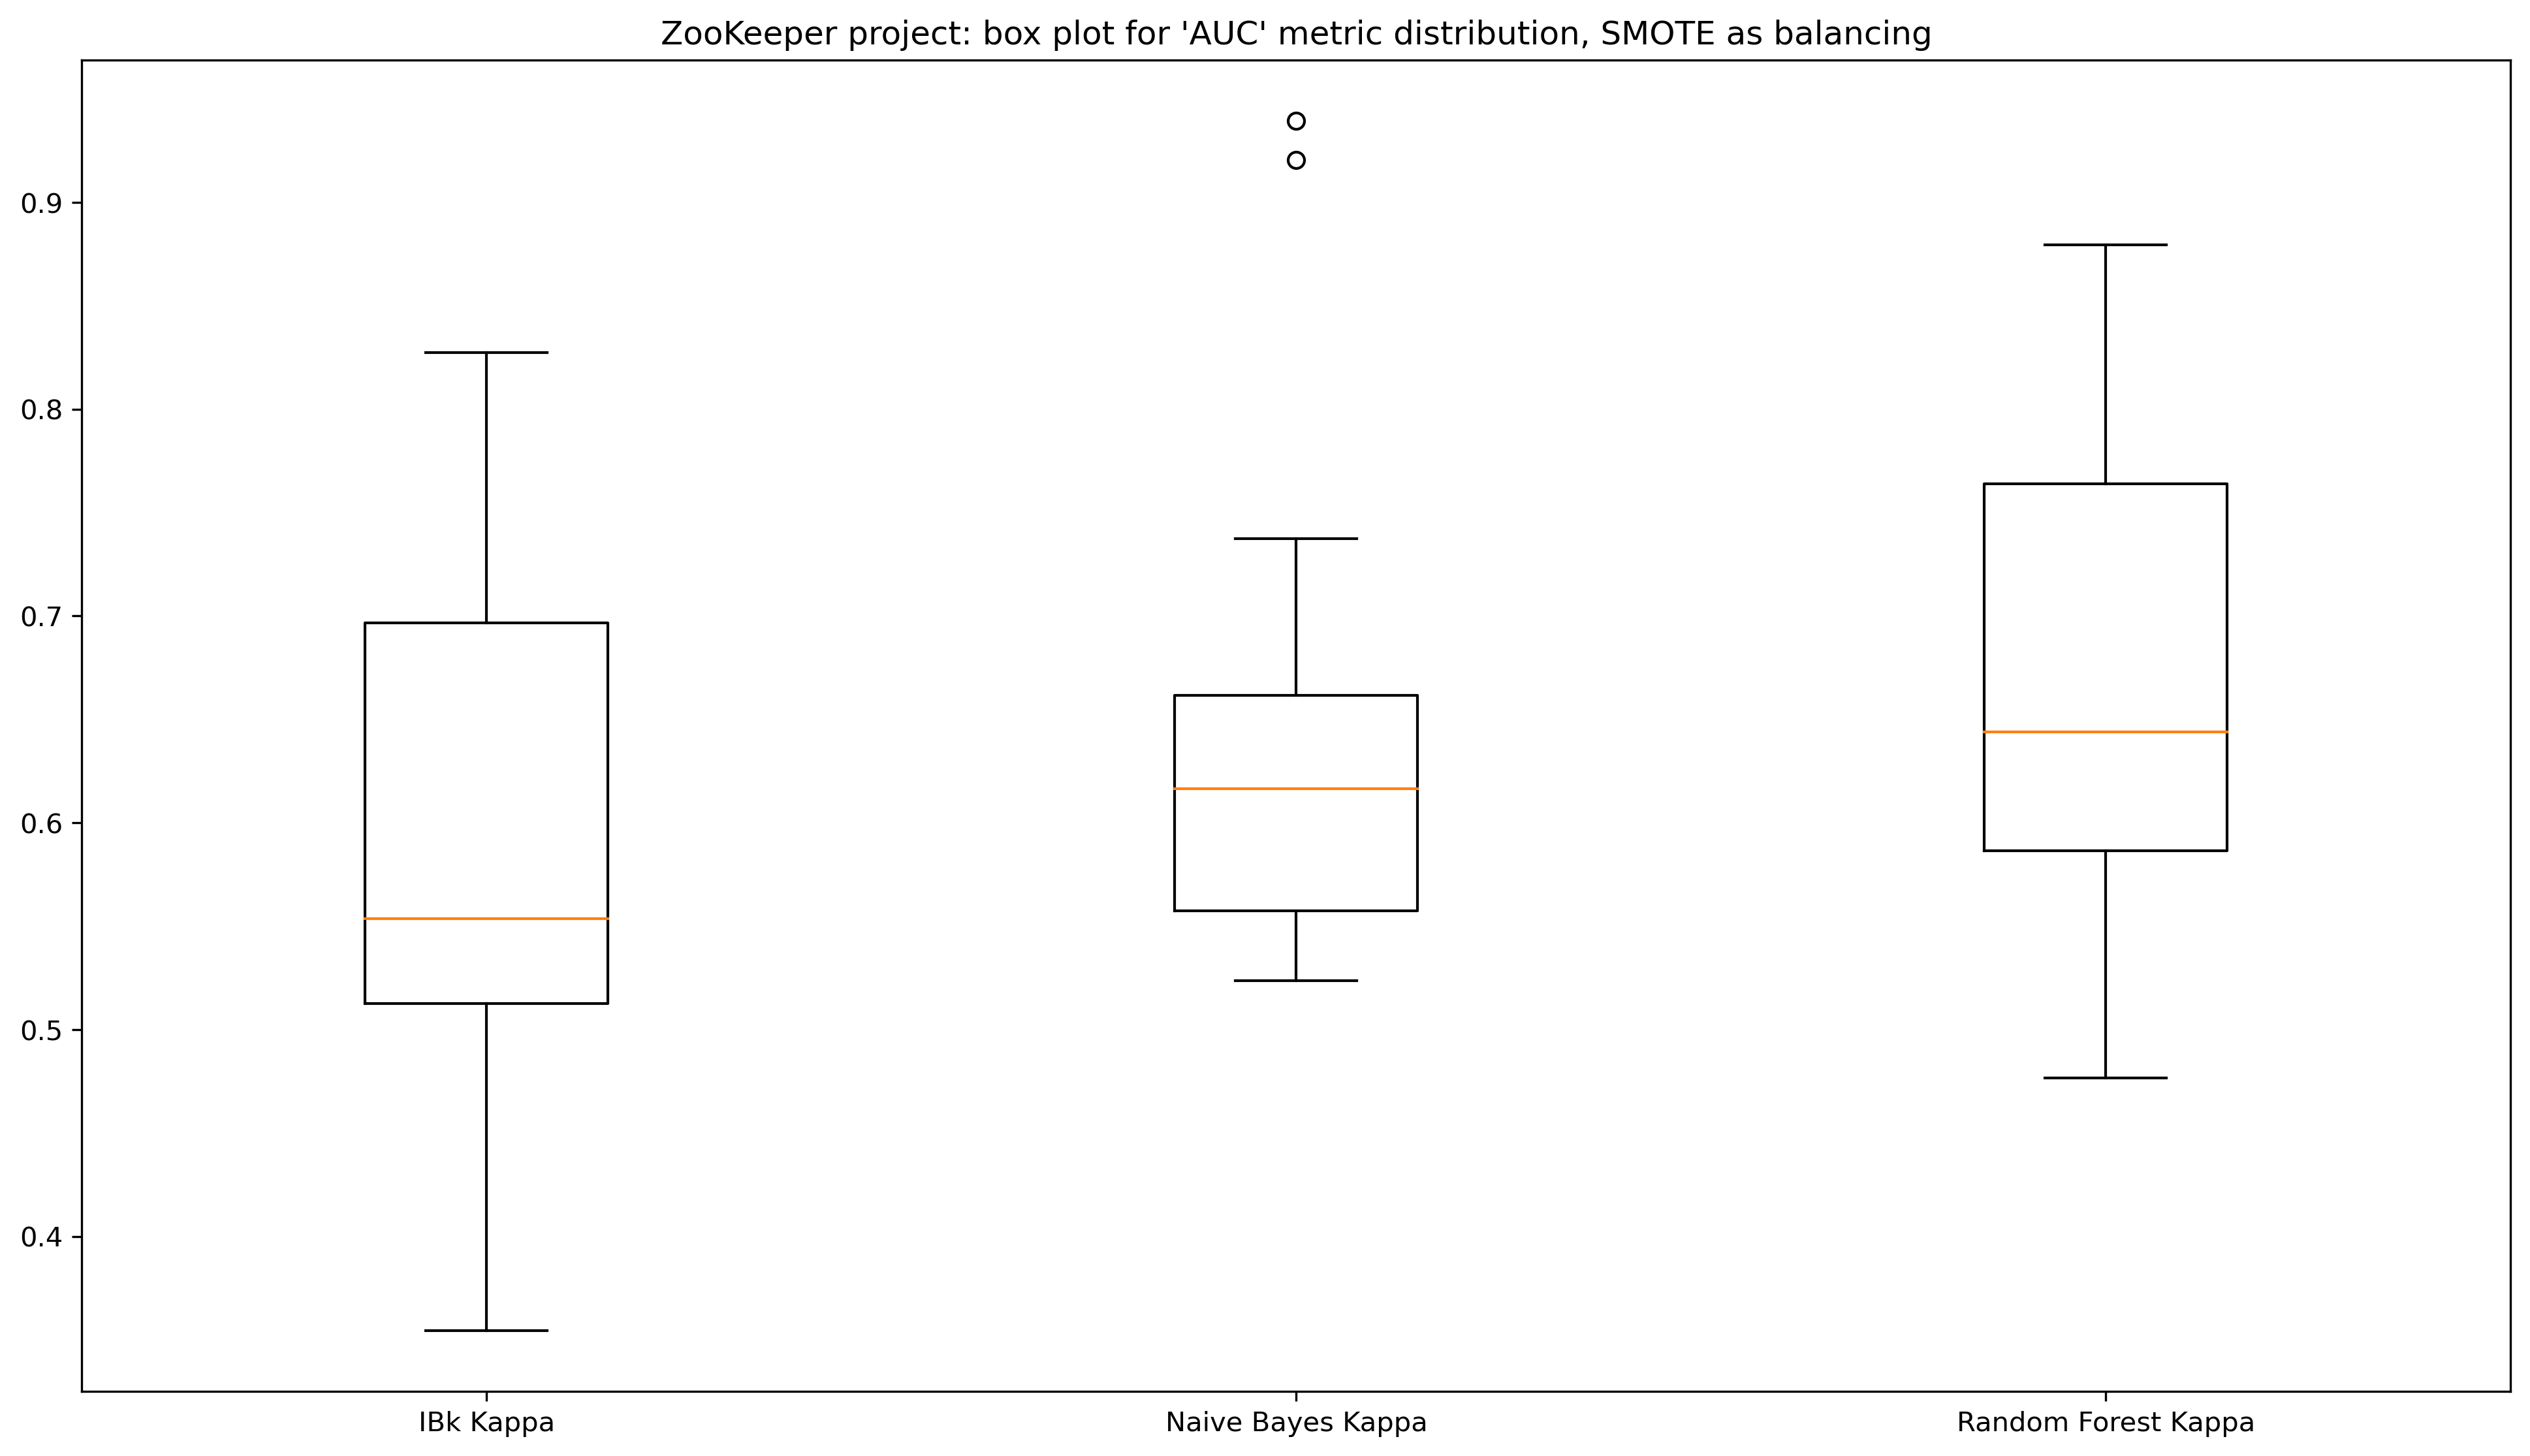
\includegraphics[scale=0.25]{images/auc_bett_zk}
\end{figure}
\end{itemize}
\end{frame}

\begin{frame}
\section{Medie dei valori per AUC}
\frametitle{Medie dei valori per AUC}
\begin{minipage}[t]{0.5\textwidth}%
\begin{figure}
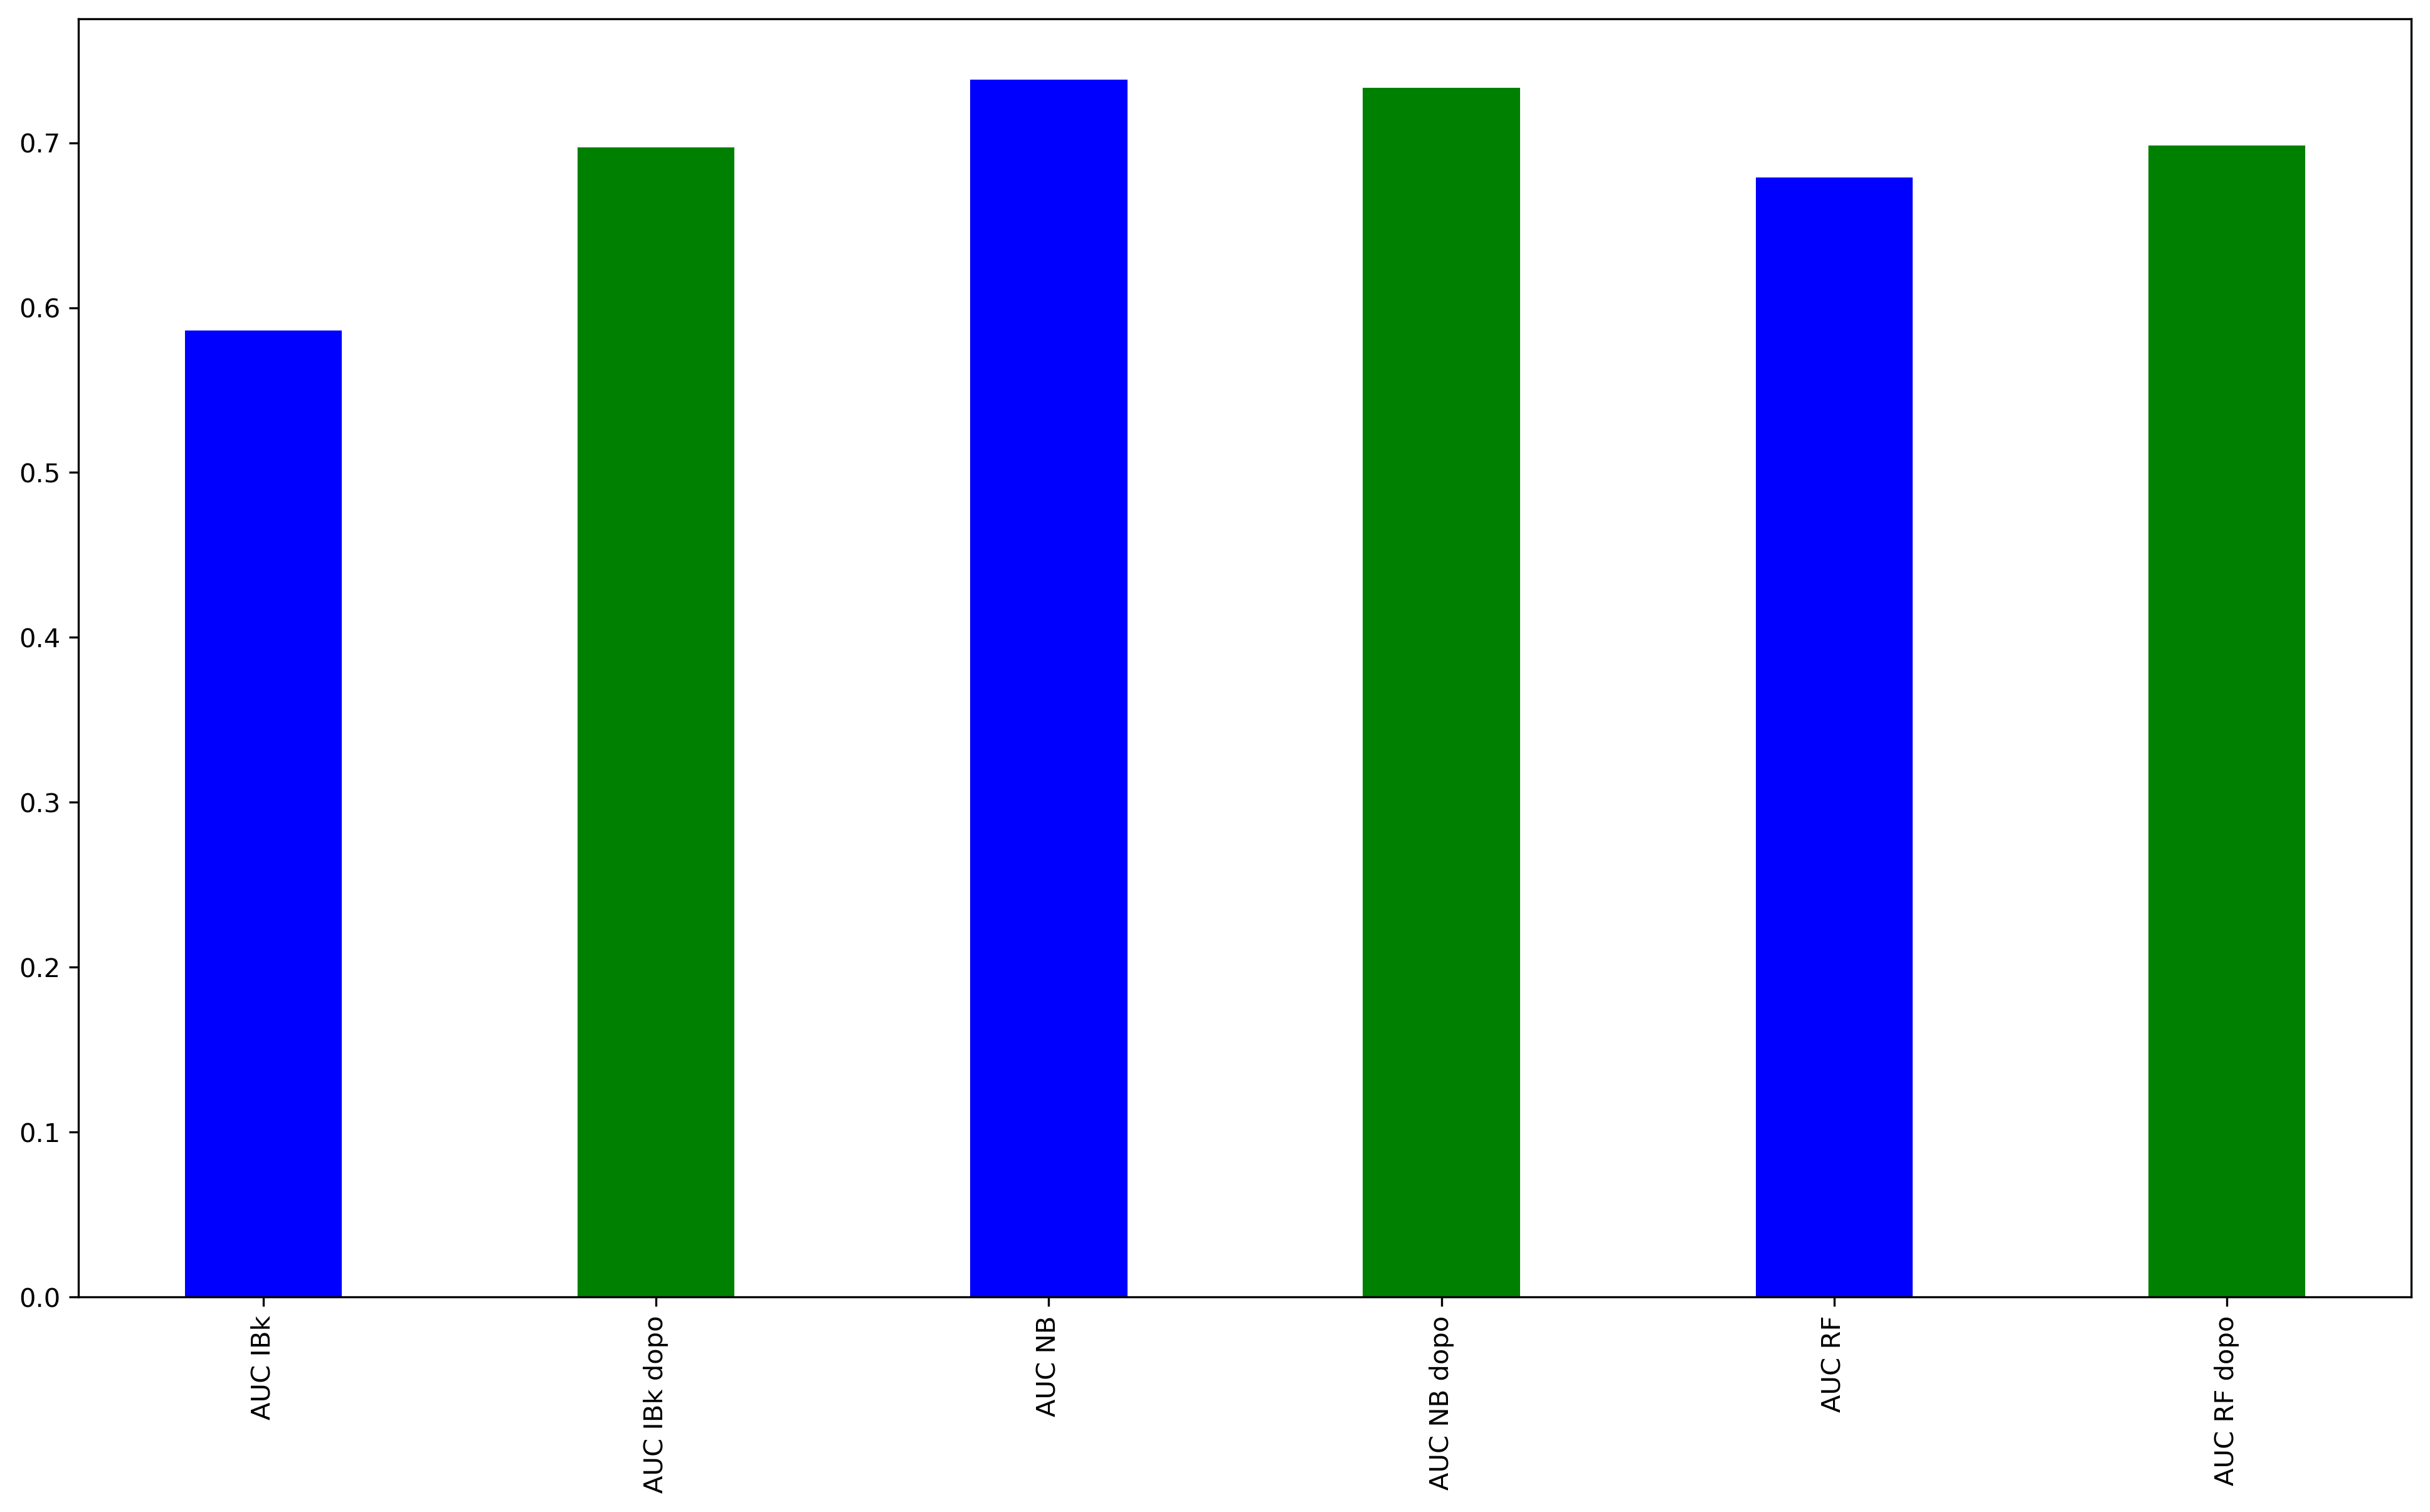
\includegraphics[scale=0.18]{images/auc_bar_bk}
\caption{Confronto dei valori di AUC per il progetto BookKeeper}
\end{figure}
\end{minipage}%
\begin{minipage}[t]{0.5\textwidth}
\begin{figure}
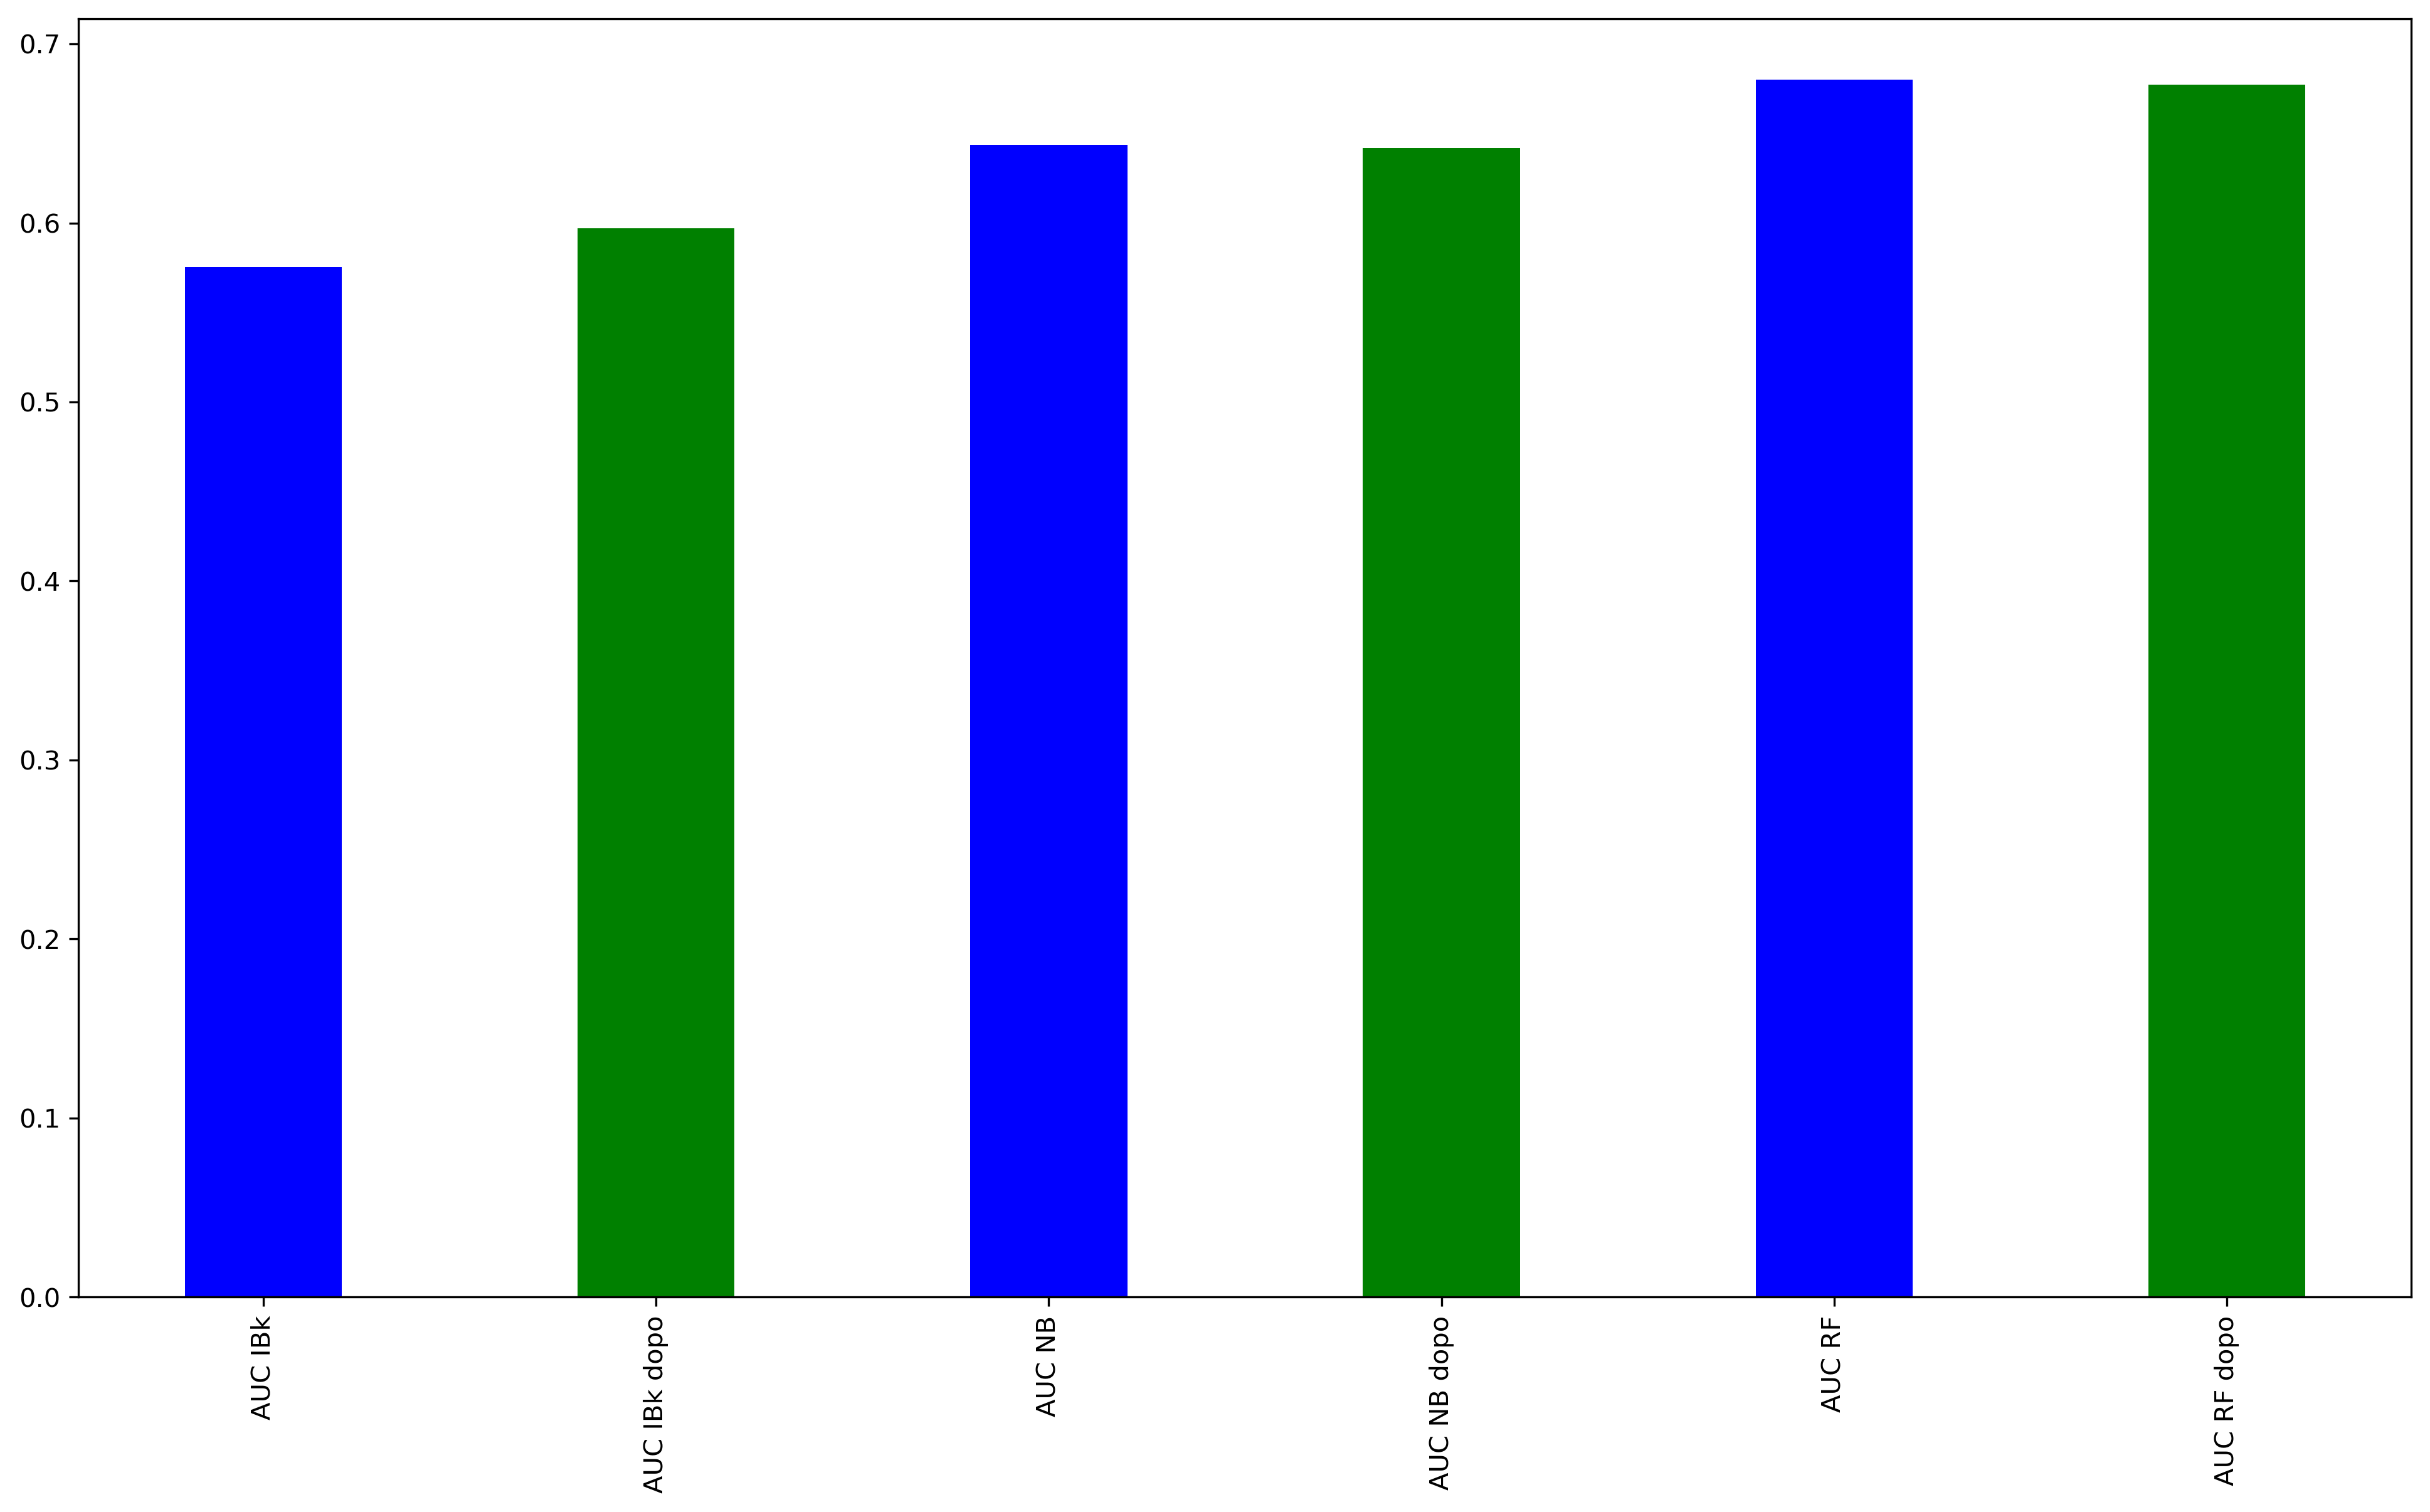
\includegraphics[scale=0.18]{images/auc_bar_zk}
\caption{Confronto dei valori di AUC per il progetto ZooKeeper}
\end{figure}
\end{minipage}
\end{frame}

\begin{frame}
\section{Analisi di Precision e Recall per BooKeeper}
\frametitle{Analisi di Precision e Recall per BookKeeper}
\begin{itemize}
\item Per il progetto BookKeeper, si ottengono i seguenti risultati:
\begin{figure}
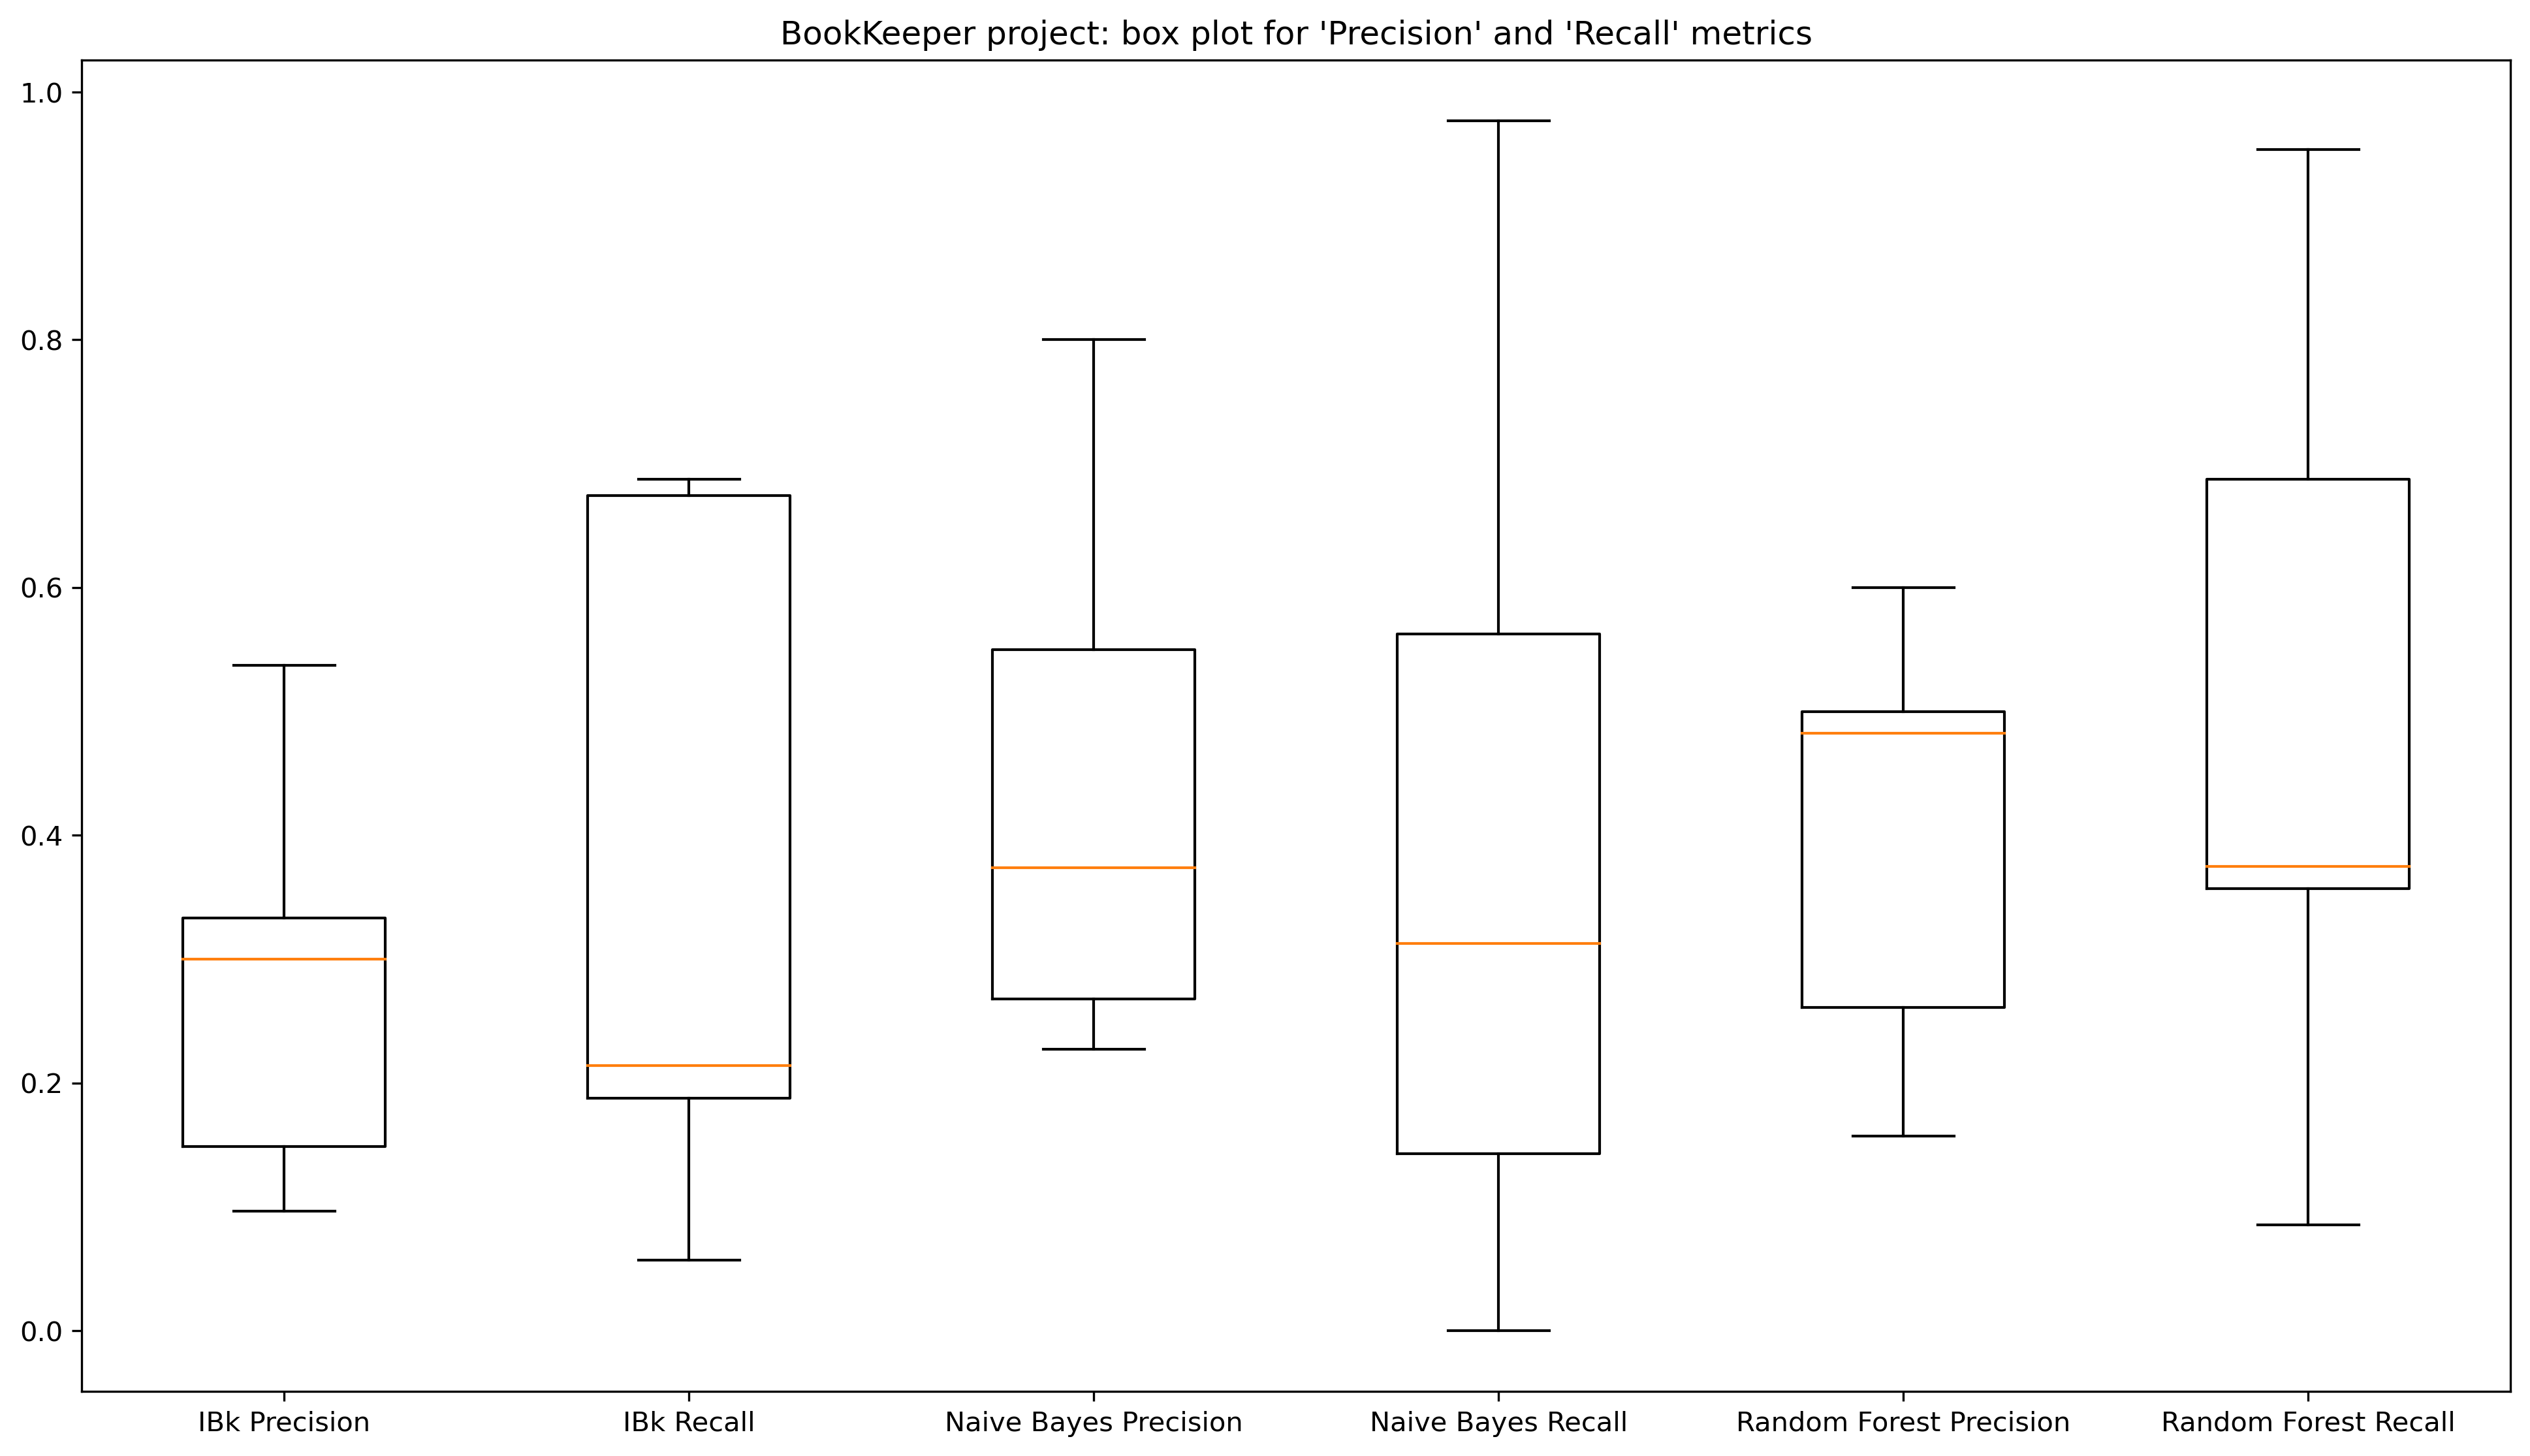
\includegraphics[scale=0.25]{images/pc_rc_base_bk}
\end{figure}
\item Tutti i classificatori sembrano mostrare delle metriche coerenti col fatto che il dataset è molto sbilanciato, essendo come già detto molto più presenti i valori "no" per l'attributo buggyness, che è quello che viene stimato
\item Questo giustifica i bassi valori di Precision, in quanto riuscire a predirre correttamente una istanza positiva non è semplice, ed anche di Recall
\end{itemize}
\end{frame}
\begin{frame}
\subsection{Tentativo di miglioramento dei valori}
\frametitle{Tentativo di miglioramento dei valori}
\begin{itemize}
\item Dall'analisi dei valori, si evince che applicando over sampling come meccanismo di balancing, feature selection e sensitive threshold, c'è una aumento molto importante dei valori delle distribuzioni per le metriche di Recall ottenute da Naive Bayes e Random Forest
\begin{figure}
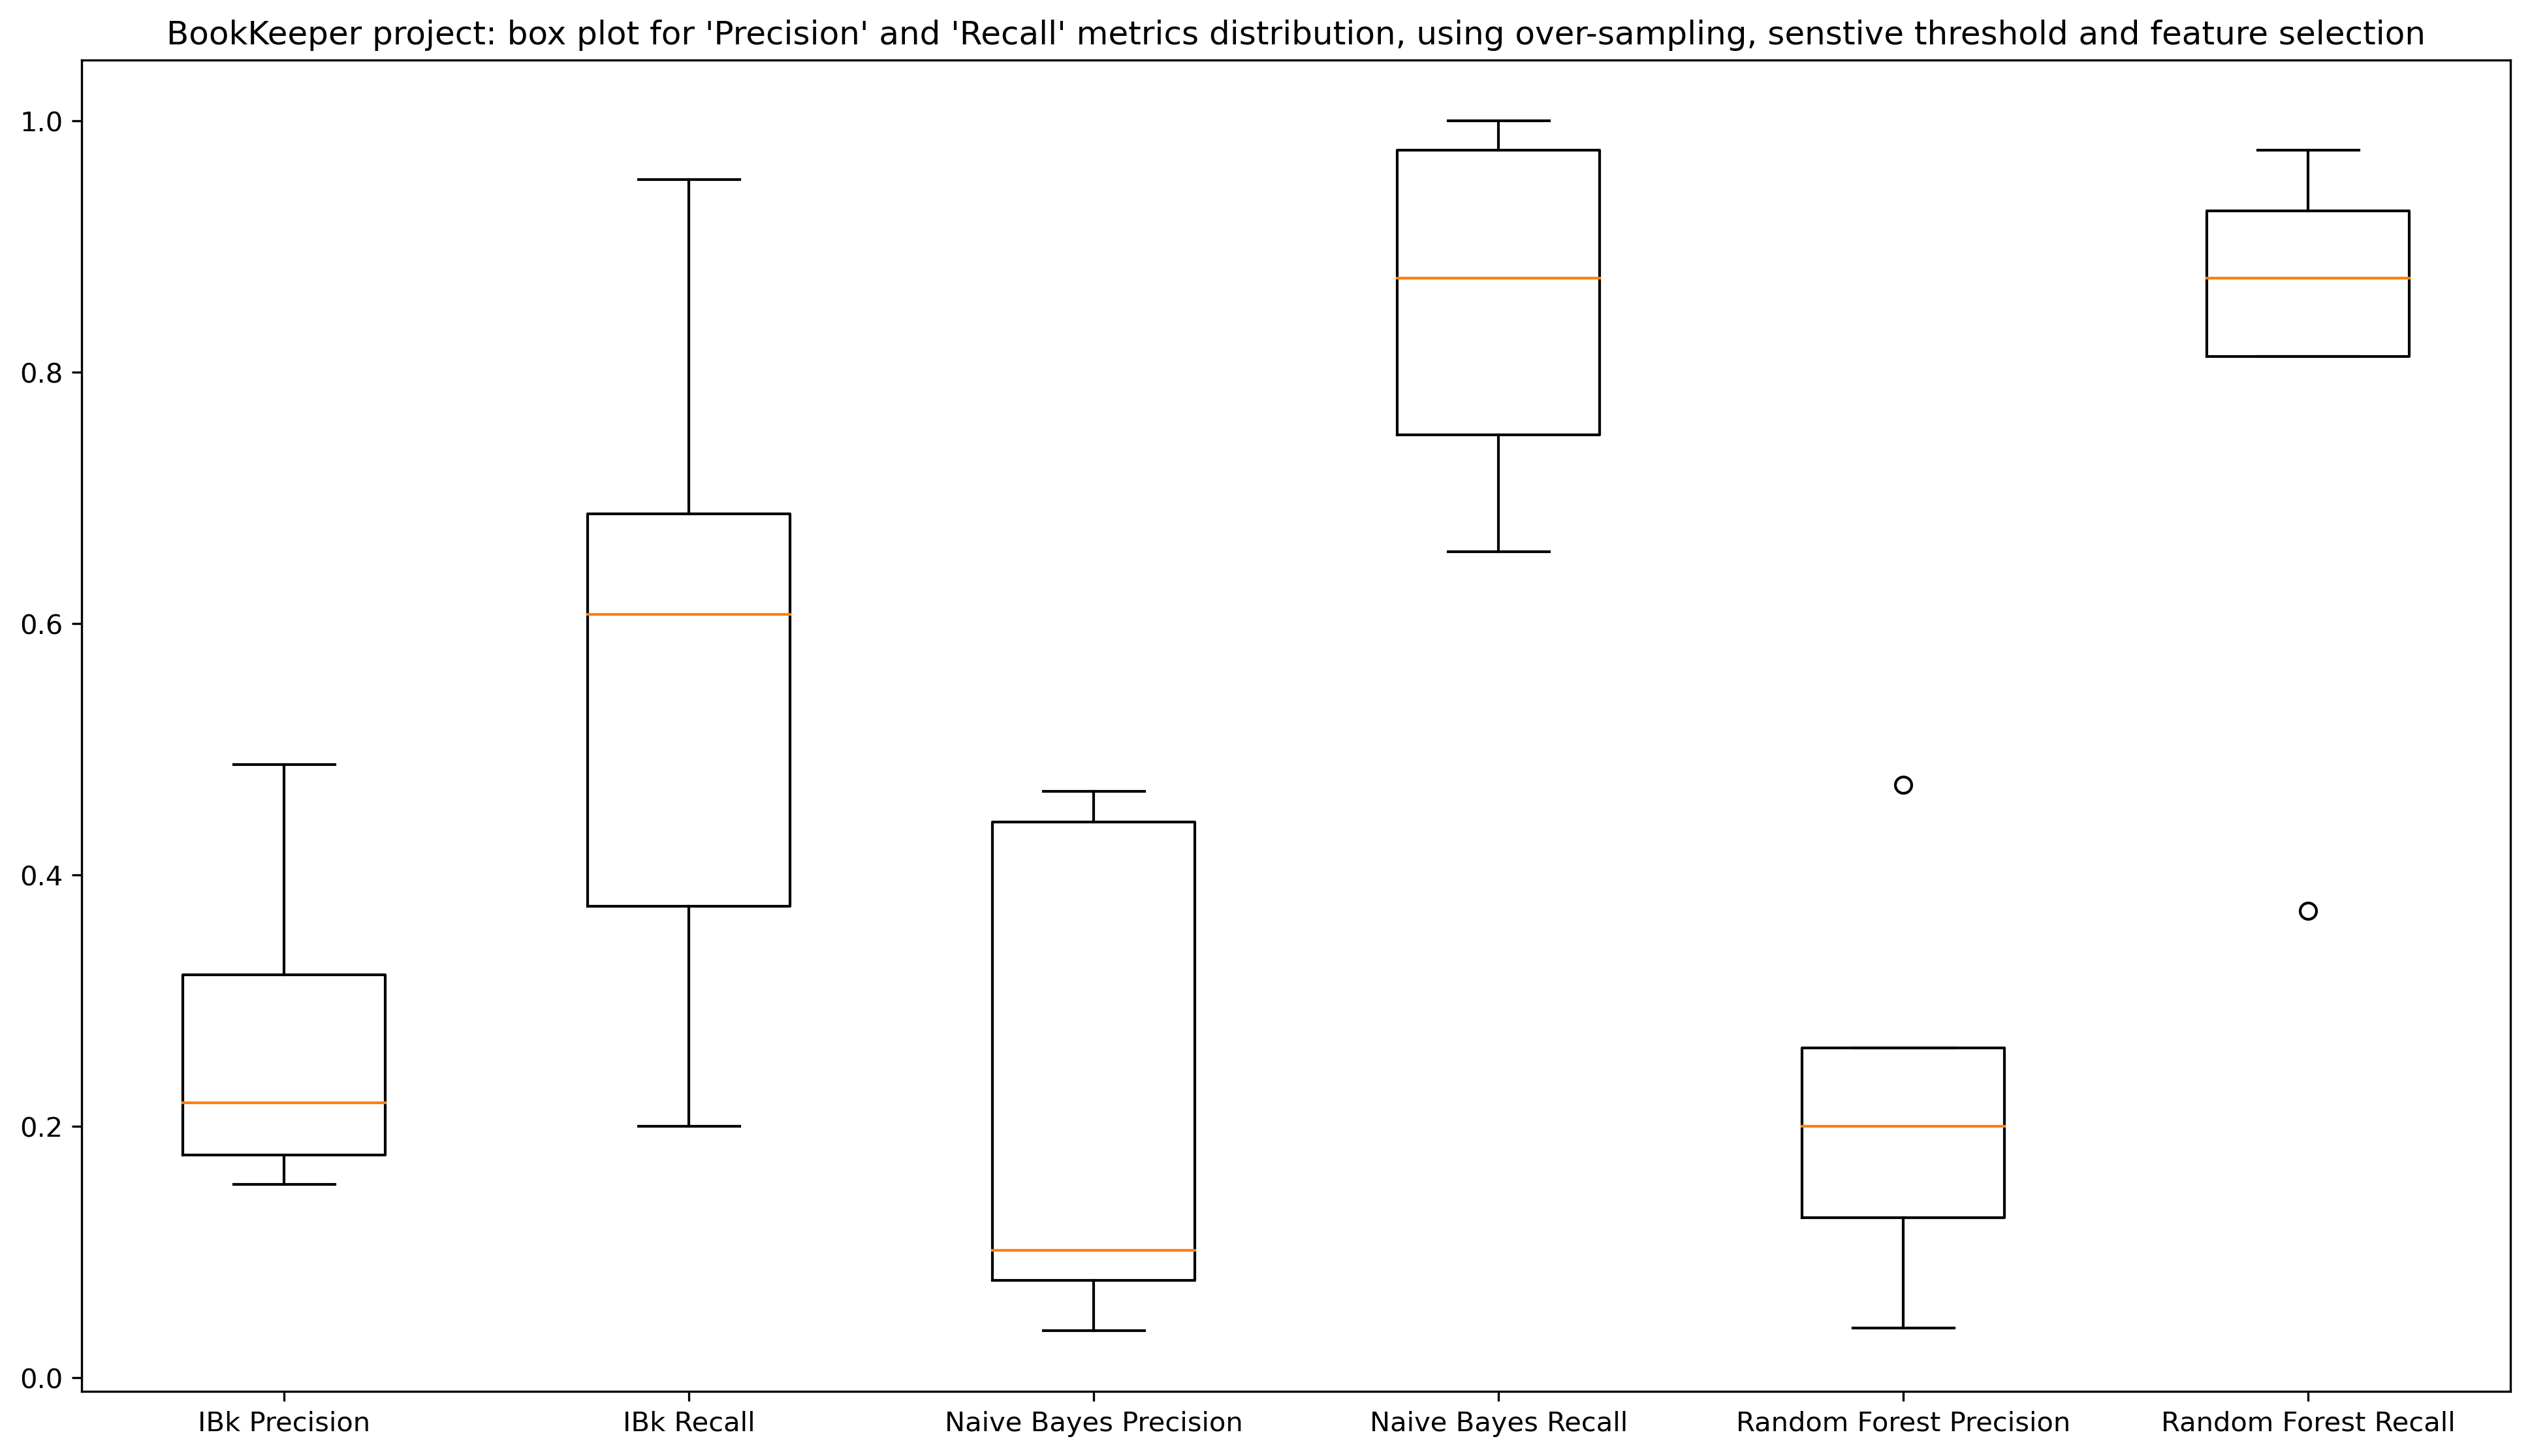
\includegraphics[scale=0.25]{images/pc_rc_2_bk}
\end{figure}
\item Avendo applicato over sampling, le istanze nella classe minoritaria stata aumentate e quindi questo spiega il vertiginoso aumento dei valori per le distribuzioni
\item I valori di Precision si abbassano rispetto al caso precedente, questo in poiché c'è un elevato numero di istanze classificate come FP
\end{itemize}
\end{frame}

\begin{frame}
\section{Analisi di Precision e Recall per ZooKeeper}
\frametitle{Analisi di Precision e Recall per ZooKeeper}
\begin{itemize}
\item Per il progetto ZooKeeper, si ottengono i seguenti risultati:
\begin{figure}
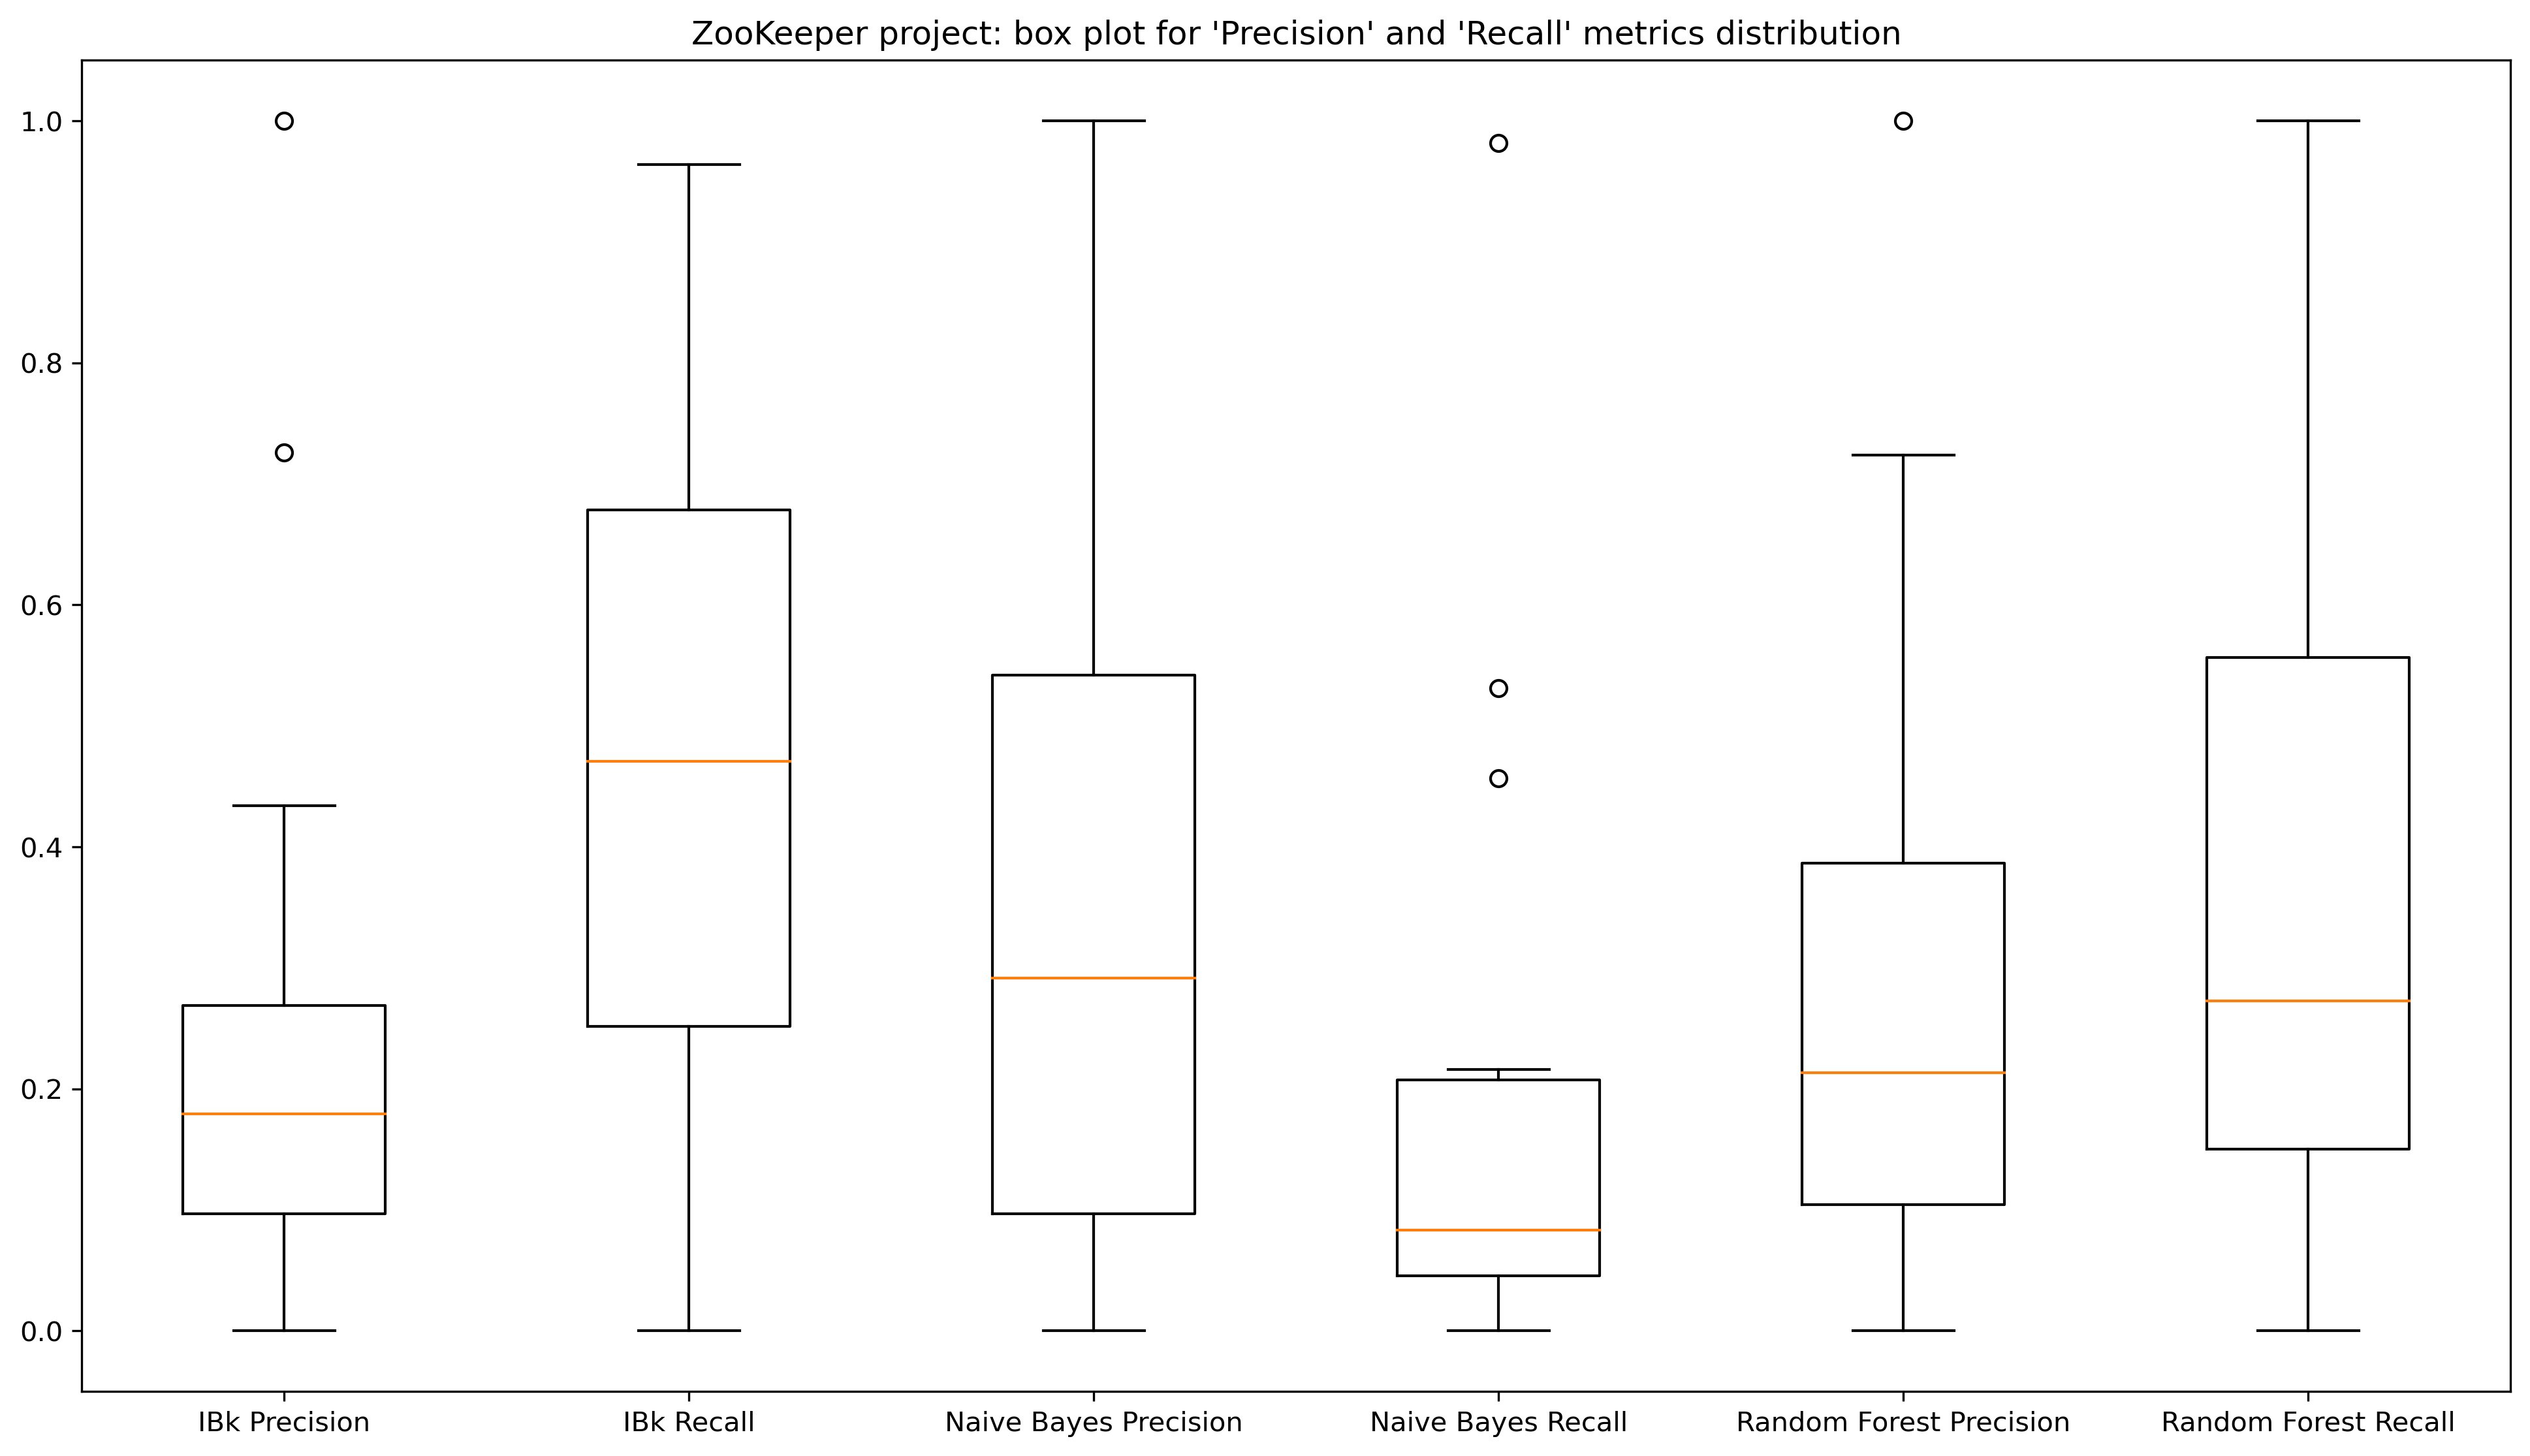
\includegraphics[scale=0.25]{images/pr_rc_base_zk}
\end{figure}
\item In questo caso, il classificatore che mostra i valori peggiori per la metrica di Precision è Naive Bayes, ma con dei valori di Recall più alti rispetto agli altri classificatori
\item Anche qui, l'obiettivo è quello di cercare di alzare i valori per le metriche di tutti i classificatori
\end{itemize}
\end{frame}
\begin{frame}
\subsection{Tentativo di miglioramento dei valori}
\frametitle{Tentativo di miglioramento dei valori}
\begin{itemize}
\item Anche in questo caso, lo scopo dell'analisi è cercare di applicare le tecniche viste per aumentare i valori di Precision e Recall
\item Applicando feature selection, sensitive threshold e SMOTE come filtro di balancing, si ottengono dei valori di Precision più alti per i classificatori IBk e Random Forest, ma la Recall rimane bassa
\begin{figure}
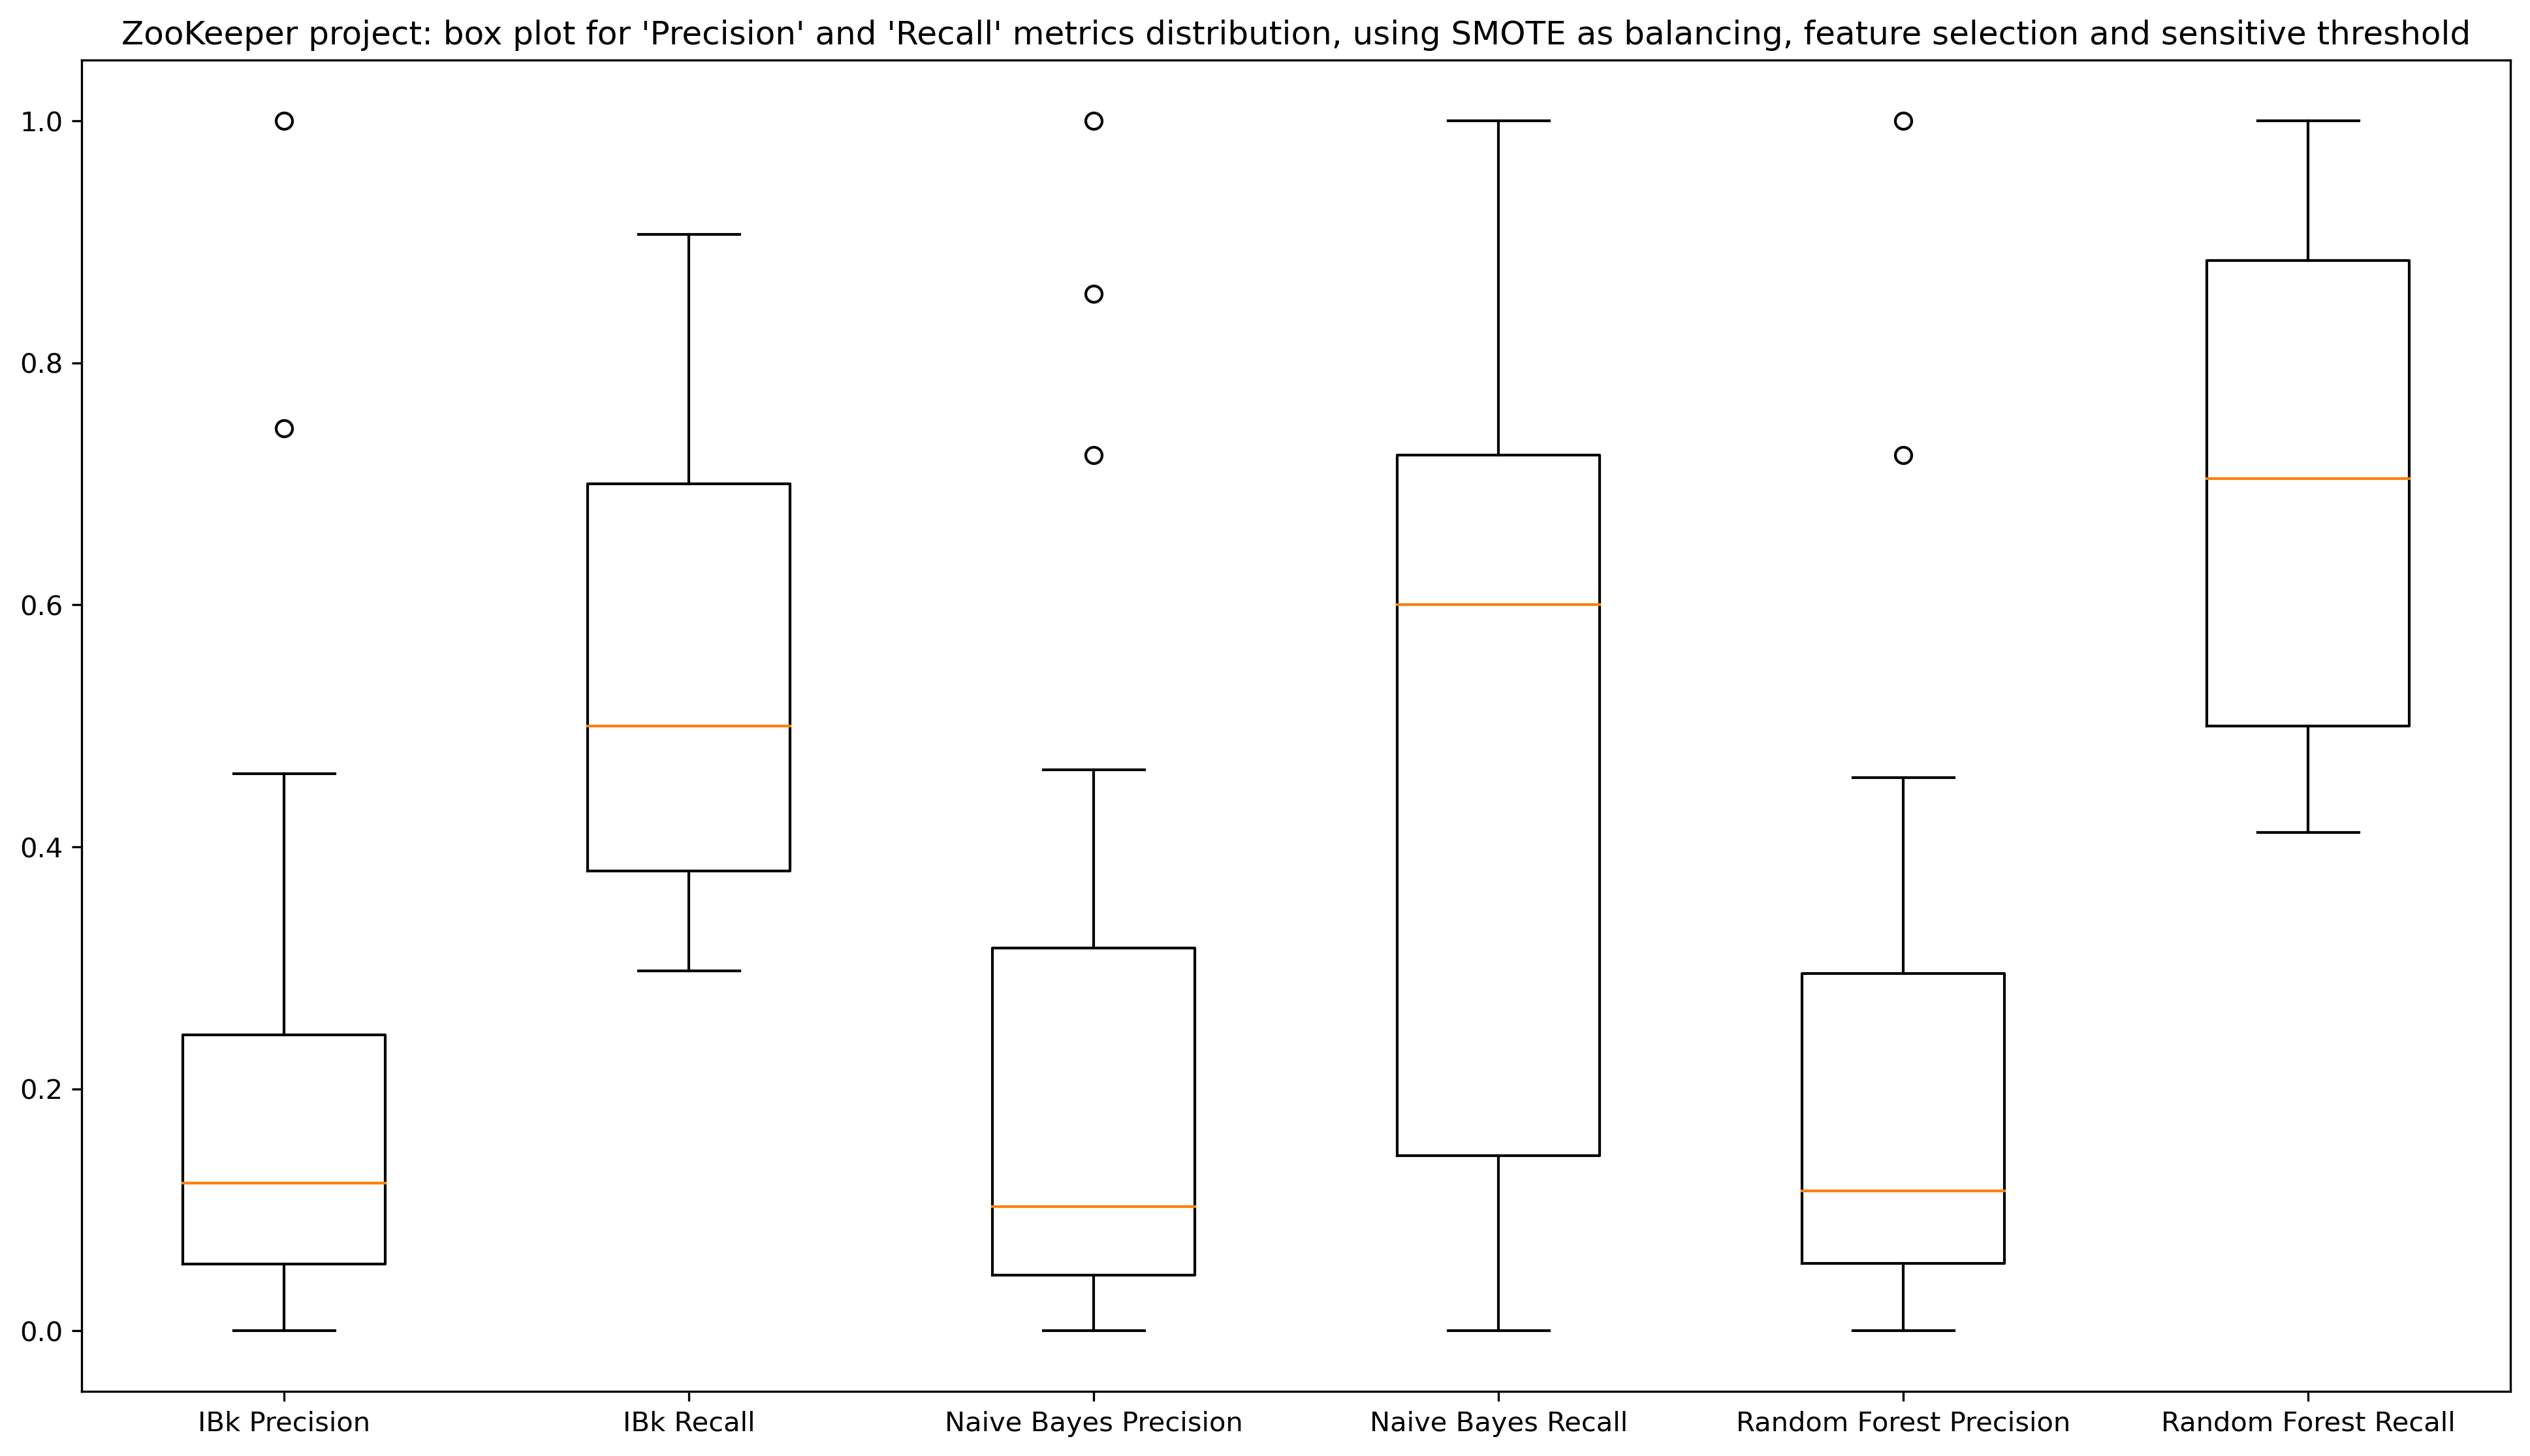
\includegraphics[scale=0.25]{images/pr_rc_bett_zk}
\end{figure}
\item la varianza per la distribuzione dei valori di Recall per Naive Bayes è molto maggiore rispetto agli altri due classificatori, quindi non c'è miglioramento 
\item Random Forest mostra una distribuzione analoga al caso precedente, ovvero senza l'applicazione di filtri, balacing o cost sensitive
\end{itemize}
\end{frame}

\begin{frame}
\section{Risultati analitici per FP - abbassamento dei valori di Precision}
\frametitle{Risultati analitici e grafici}
\begin{table}
\begin{tabular}{|c|c|c|}
\hline
Classificatore & Media dei FP & Tecniche usate\\
IBk & 18.95 & Nessuna\\
IBk & 38.68 & SMOTE + FS + Sens. Thresh.\\
\hline
Naive Bayes & 4.1 & Nessuna \\
Naive Bayes & 27.22 & SMOTE + FS + Sens. Thresh.\\
\hline
Random Forest & 13.13 & Nessuna \\
Random Forest & 48.12 & SMOTE + FS + Sens. Thresh.\\
\hline
\end{tabular}
\caption{Valori medi dei FP per il progetto ZooKeeper prima e dopo l'applicazione delle tecniche}
\end{table}

\begin{table}
\begin{tabular}{|c|c|c|}
\hline
Classificatore & Media dei FP & Tecniche usate\\
IBk & 8.93 & Nessuna\\
IBk & 12.53 & over-sampl. + FS + Sens. Thresh.\\
\hline
Naive Bayes & 5.93 & Nessuna \\
Naive Bayes & 56.07 & over-sampl. + FS + Sens. Thresh.\\
\hline
Random Forest & 8.8 & Nessuna \\
Random Forest & 38.87 & over-sampl. + FS + Sens. Thresh.\\
\hline
\end{tabular}
\caption{Valori medi dei FP per il progetto BookKeeper prima e dopo l'applicazione delle tecniche}
\end{table}
\begin{itemize}
\item I valori medi mostrano chiaramente i risultati ottenuti per Precision, ovvero l'abbassamento dei valori per tutti i classificatori
\end{itemize}
\end{frame}

\begin{frame}
\section{Analisi di Kappa per BookKeeper}
\frametitle{Analisi di Kappa per BookKeeper}
\begin{itemize}
\item Le distribuzioni dei valori per la metrica kappa, per tutti i classificatori, sul progetto BookKeeper senza l'utilizzo delle tecniche viste in precedenza sono mostrati nel box plot sottostante
\begin{figure}
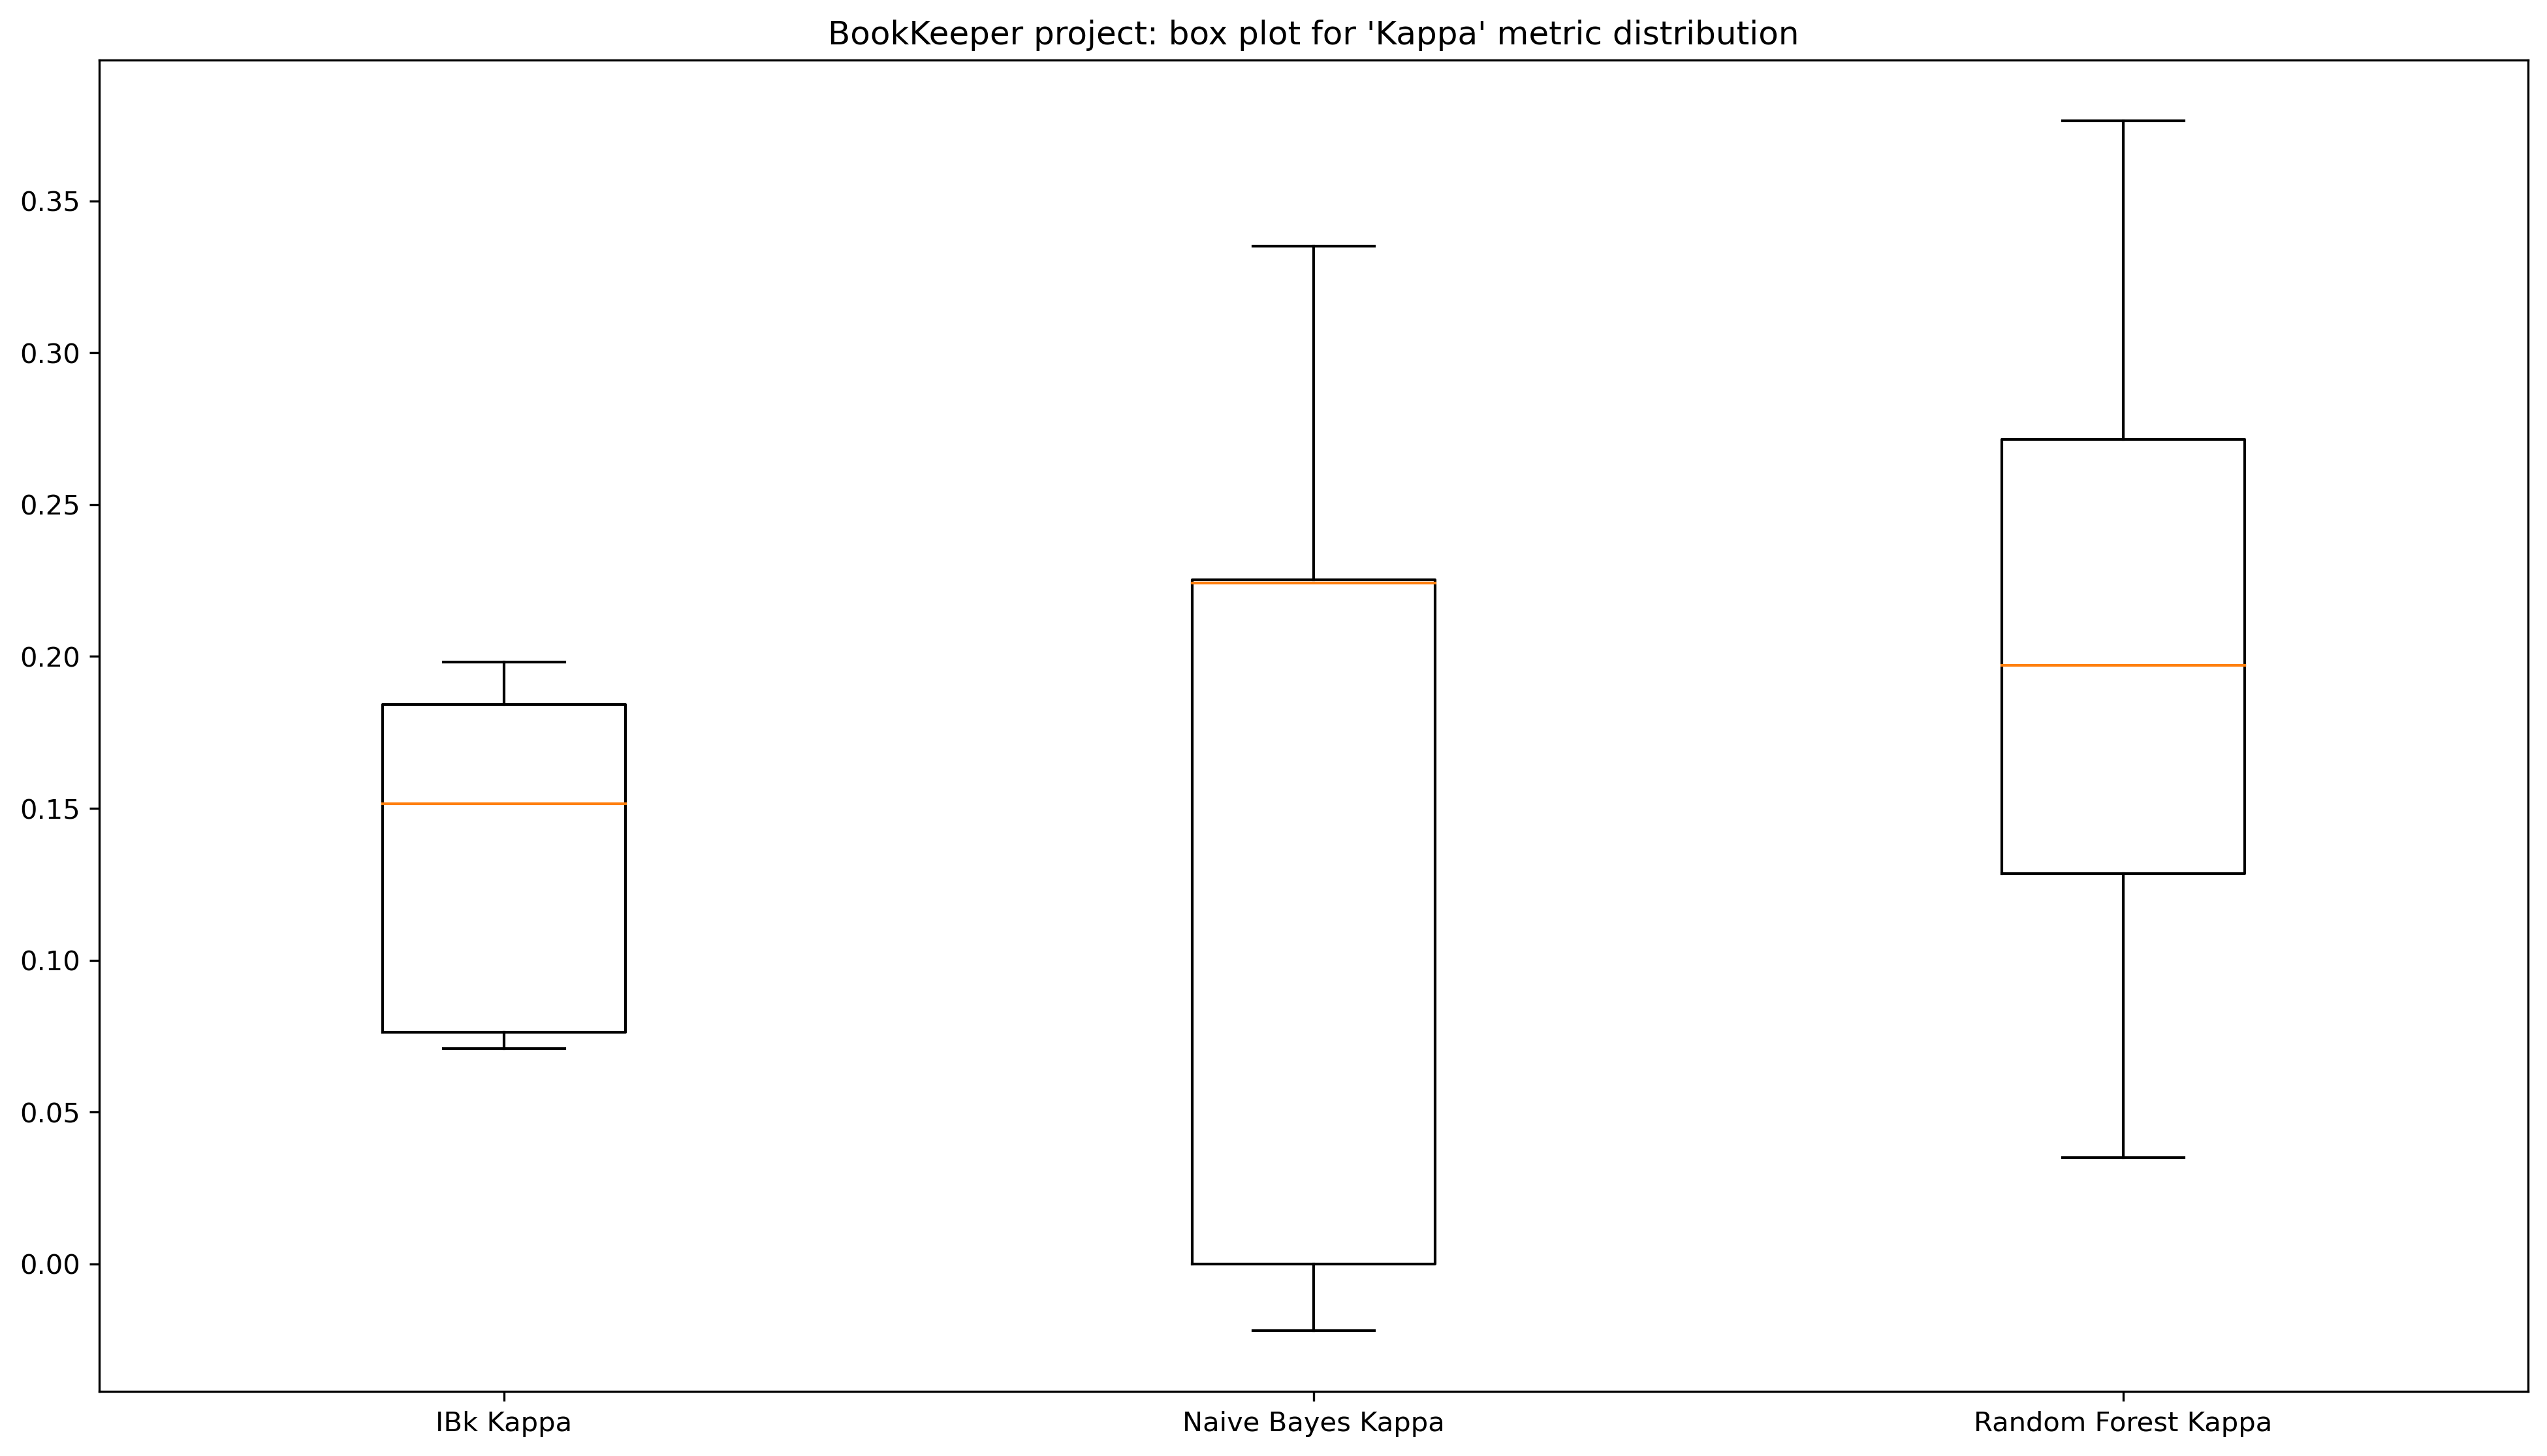
\includegraphics[scale=0.25]{images/k_base_bk}
\end{figure}
\item I classificatori che mostrano la distribuzione dei valori migliori sono IBk e Random Forest
\item Tutti i classificatori presentano dei valori che risultano, per determinate run, valori peggiori o uguali ad un classificatore random, quindi il miglioramento è stato concentrato su tale classificatore
\end{itemize}
\end{frame}

\begin{frame}
\subsection{Miglioramento dei valori di Kappa per BookKeeper}
\frametitle{Analisi di Kappa per BookKeeper}
\begin{itemize}
\item Applicando SMOTE come filtro per il sampling e feature selection, la distribuzione dei valori per la kappa ottenuta da Naive Bayes migliorano di molto, così come anche quelli di Random Forest
\begin{figure}
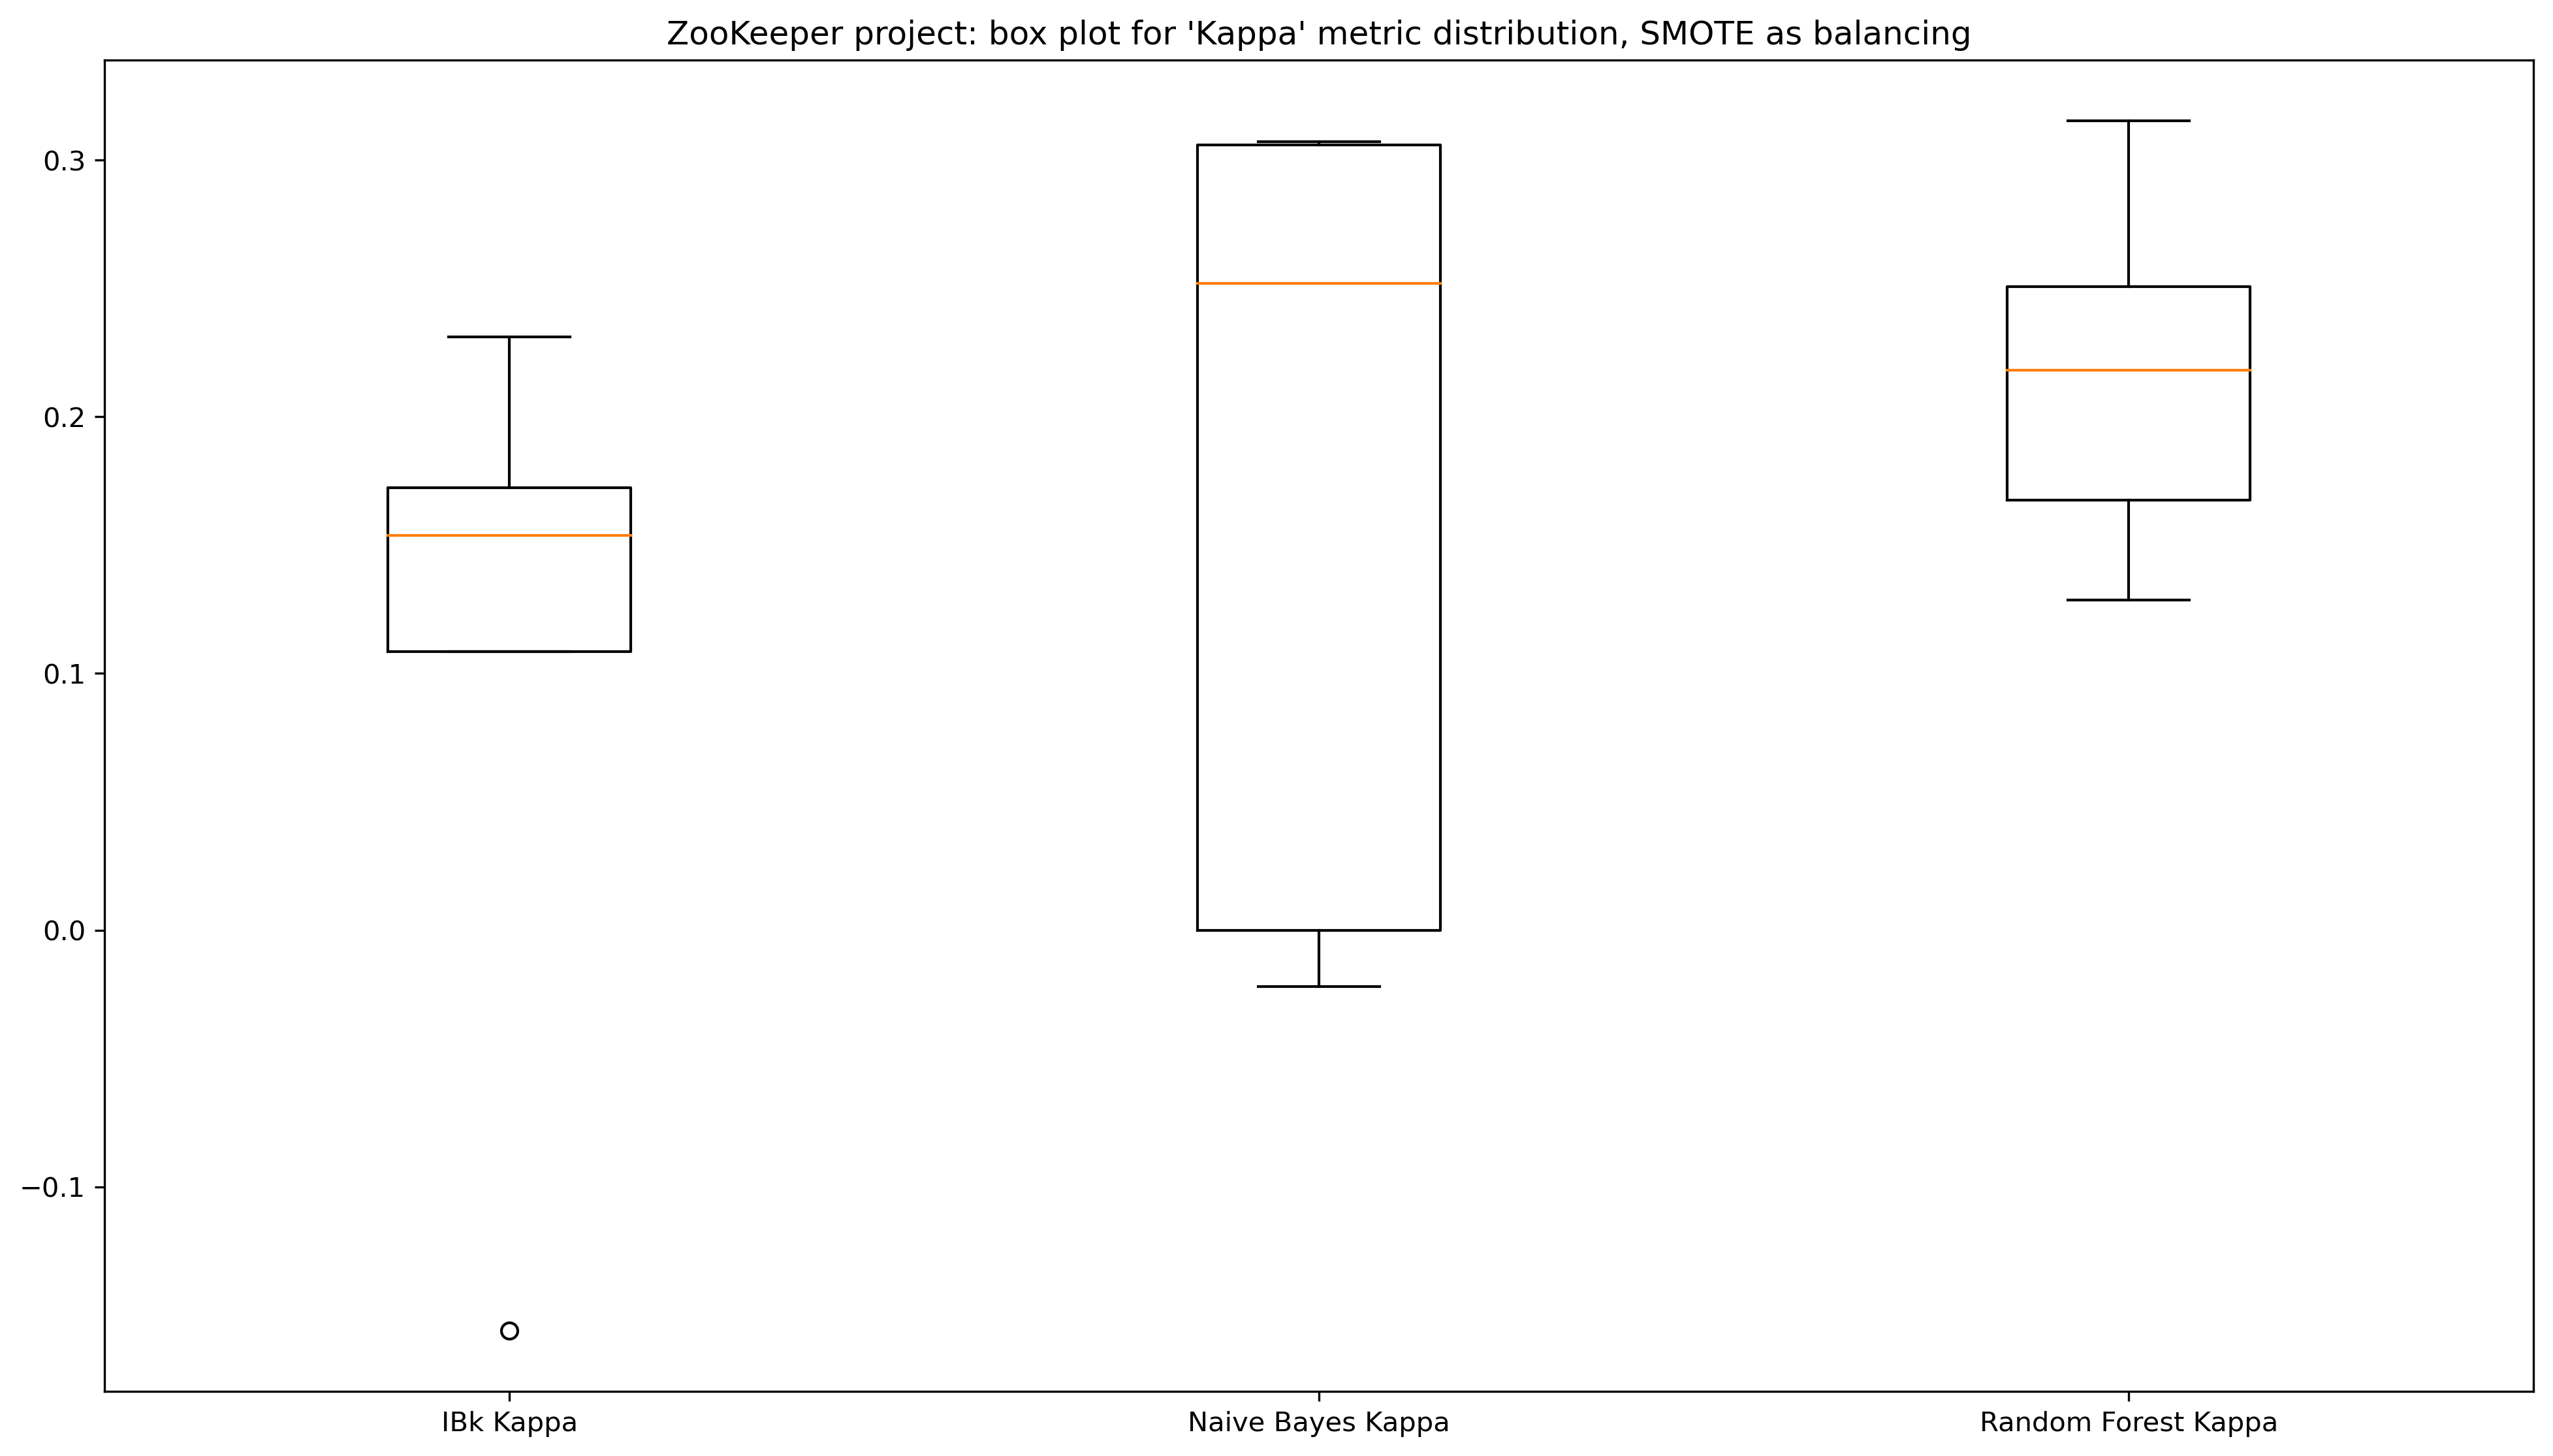
\includegraphics[scale=0.25]{images/k_bett_bk}
\end{figure}
\item Per IBk invece, viene riscontrato un peggioramento dei valori della distribuzione
\end{itemize}
\end{frame}

\begin{frame}
\section{Analisi di Kappa per ZooKeeper}
\frametitle{Analisi di Kappa per ZooKeeper}
\begin{itemize}
\item Per il progetto Zookeeper, senza l'applicazione di alcuna tecnica, si ottengono i seguenti valori
\begin{figure}
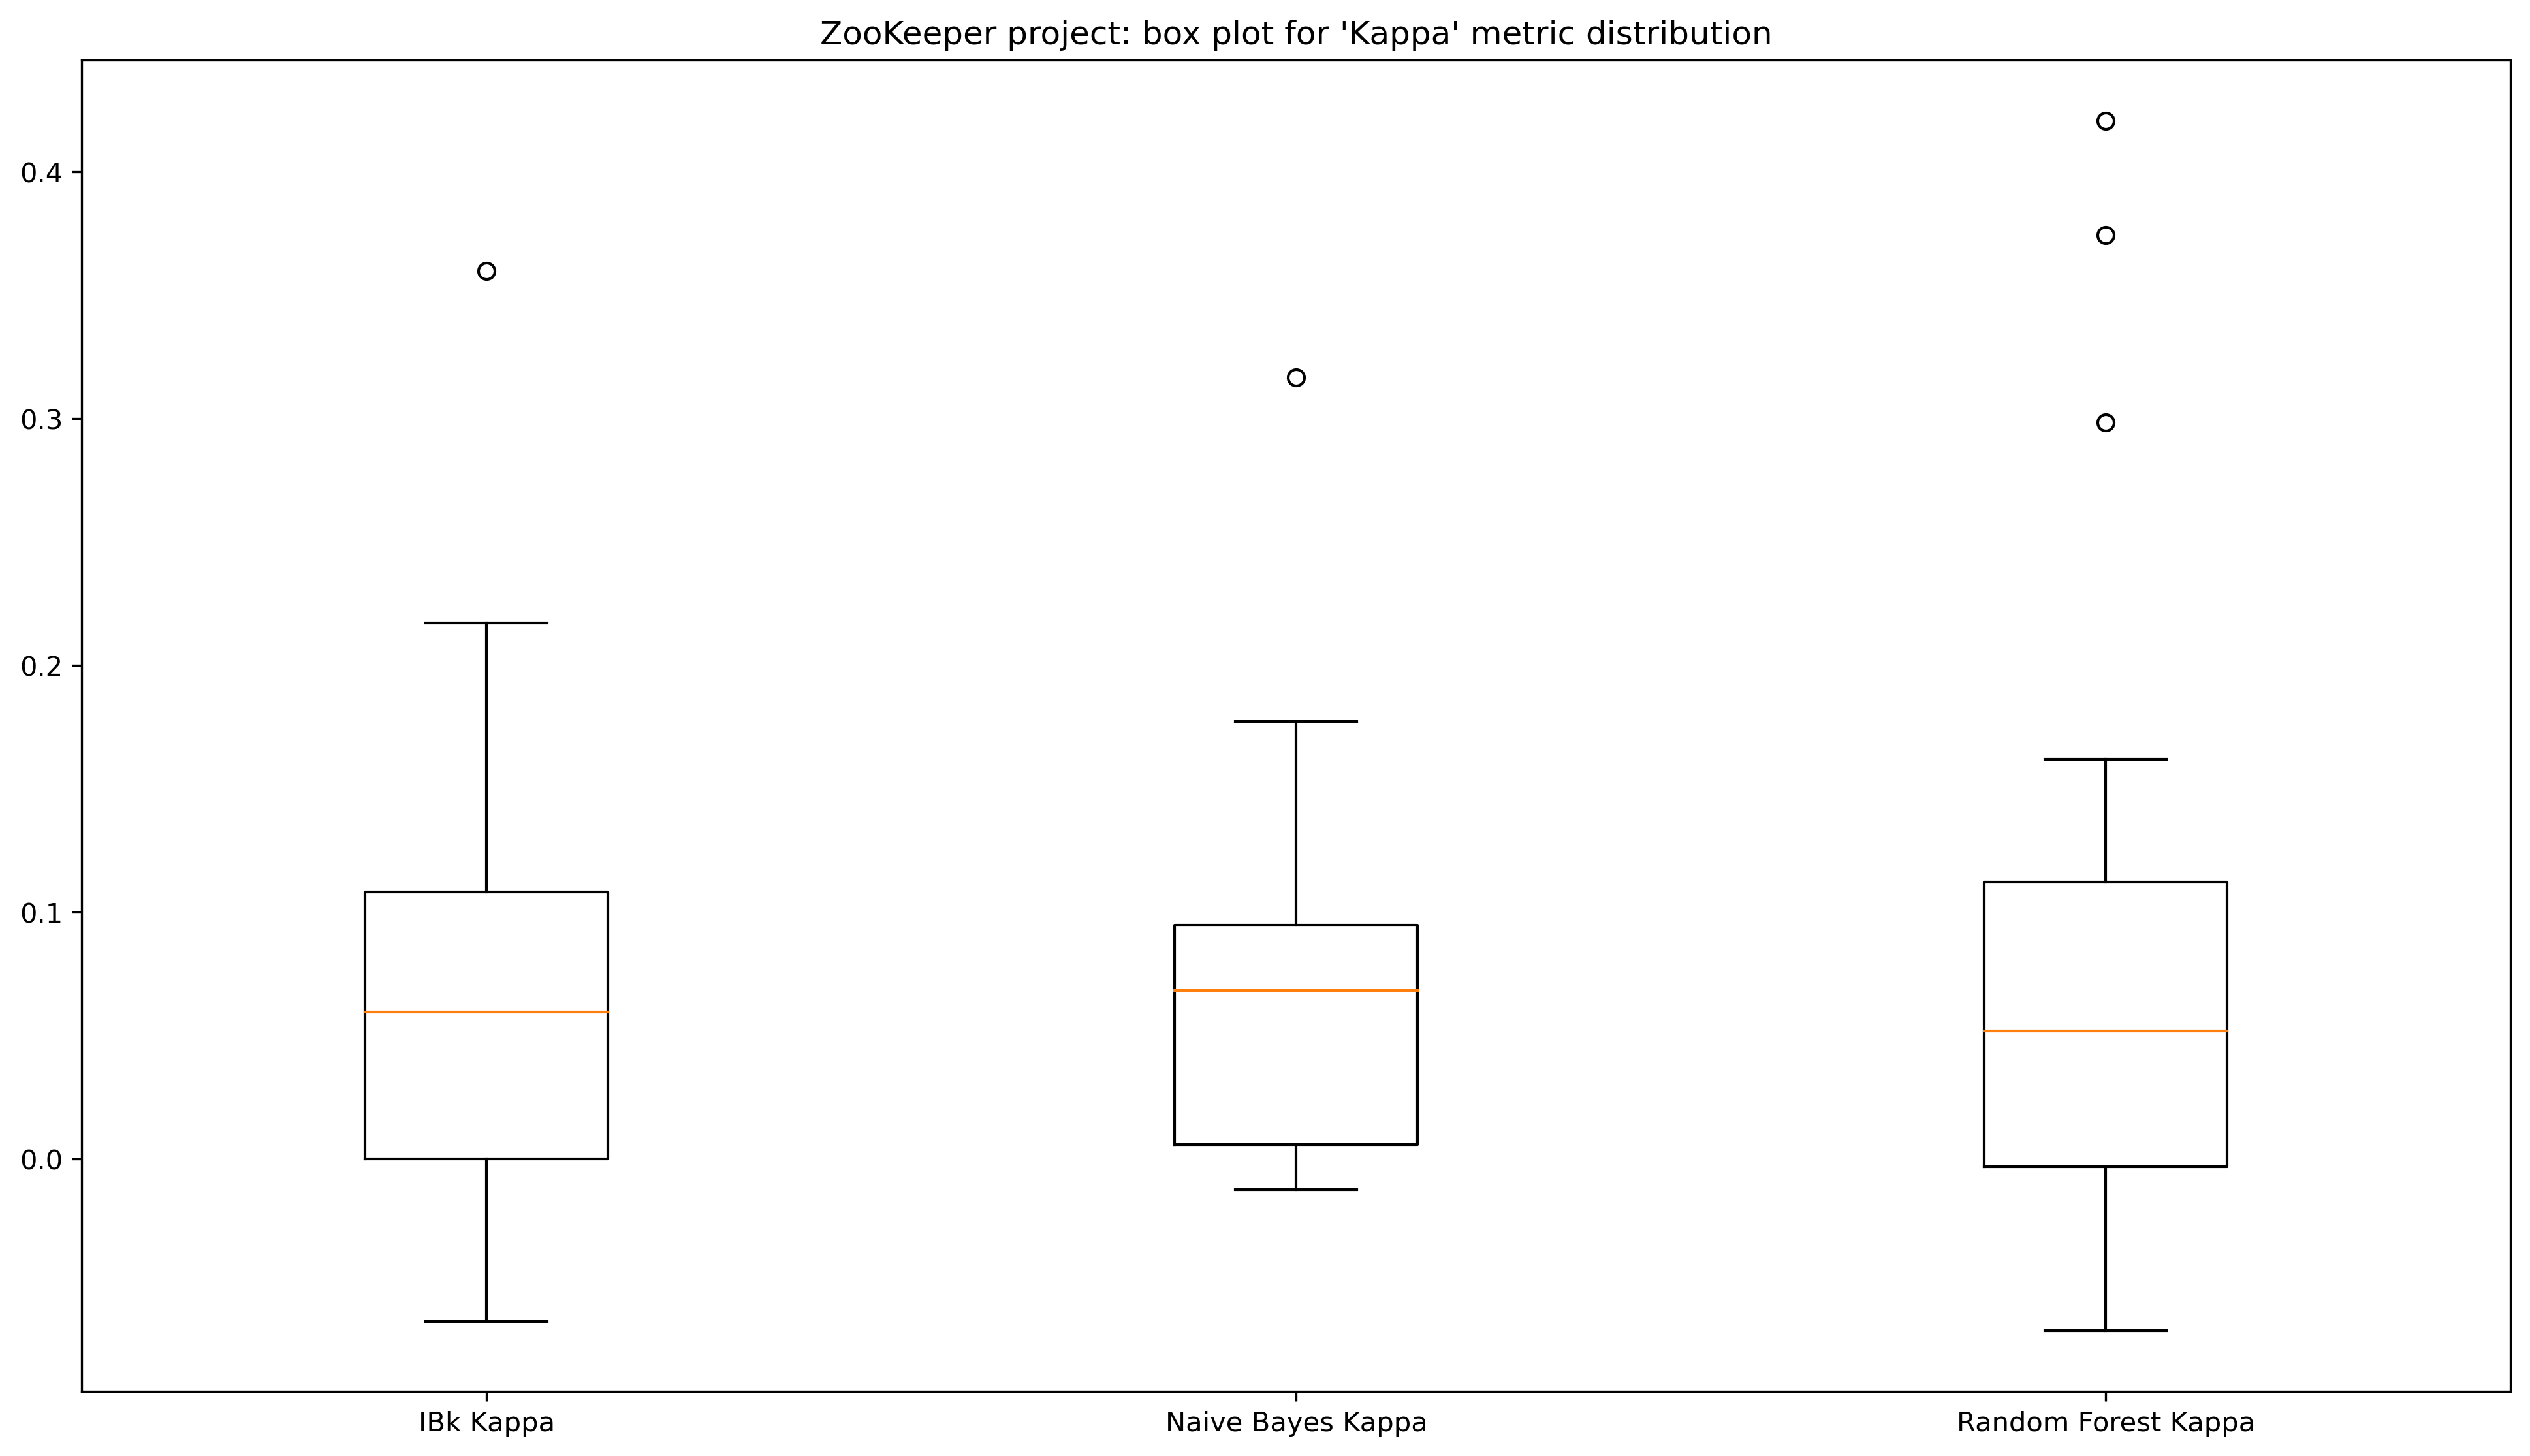
\includegraphics[scale=0.25]{images/k_base_zk}
\end{figure}
\item Per tutti i classificatori, ci sono valori della distribuzione che risultano peggiori di quanto si avrebbe con un classificatore random
\item L'obiettivo è quello di cercare di migliorare i valori per tutti e 3 i classificatori
\end{itemize}
\end{frame}

\begin{frame}
\subsection{Miglioramento dei valori}
\frametitle{Miglioramento dei valori}
\begin{itemize}
\item Applicando SMOTE come filtro per il balancing, si ottiene un modesto miglioramento nei valori per IBk e per Naive Bayes
\begin{figure}
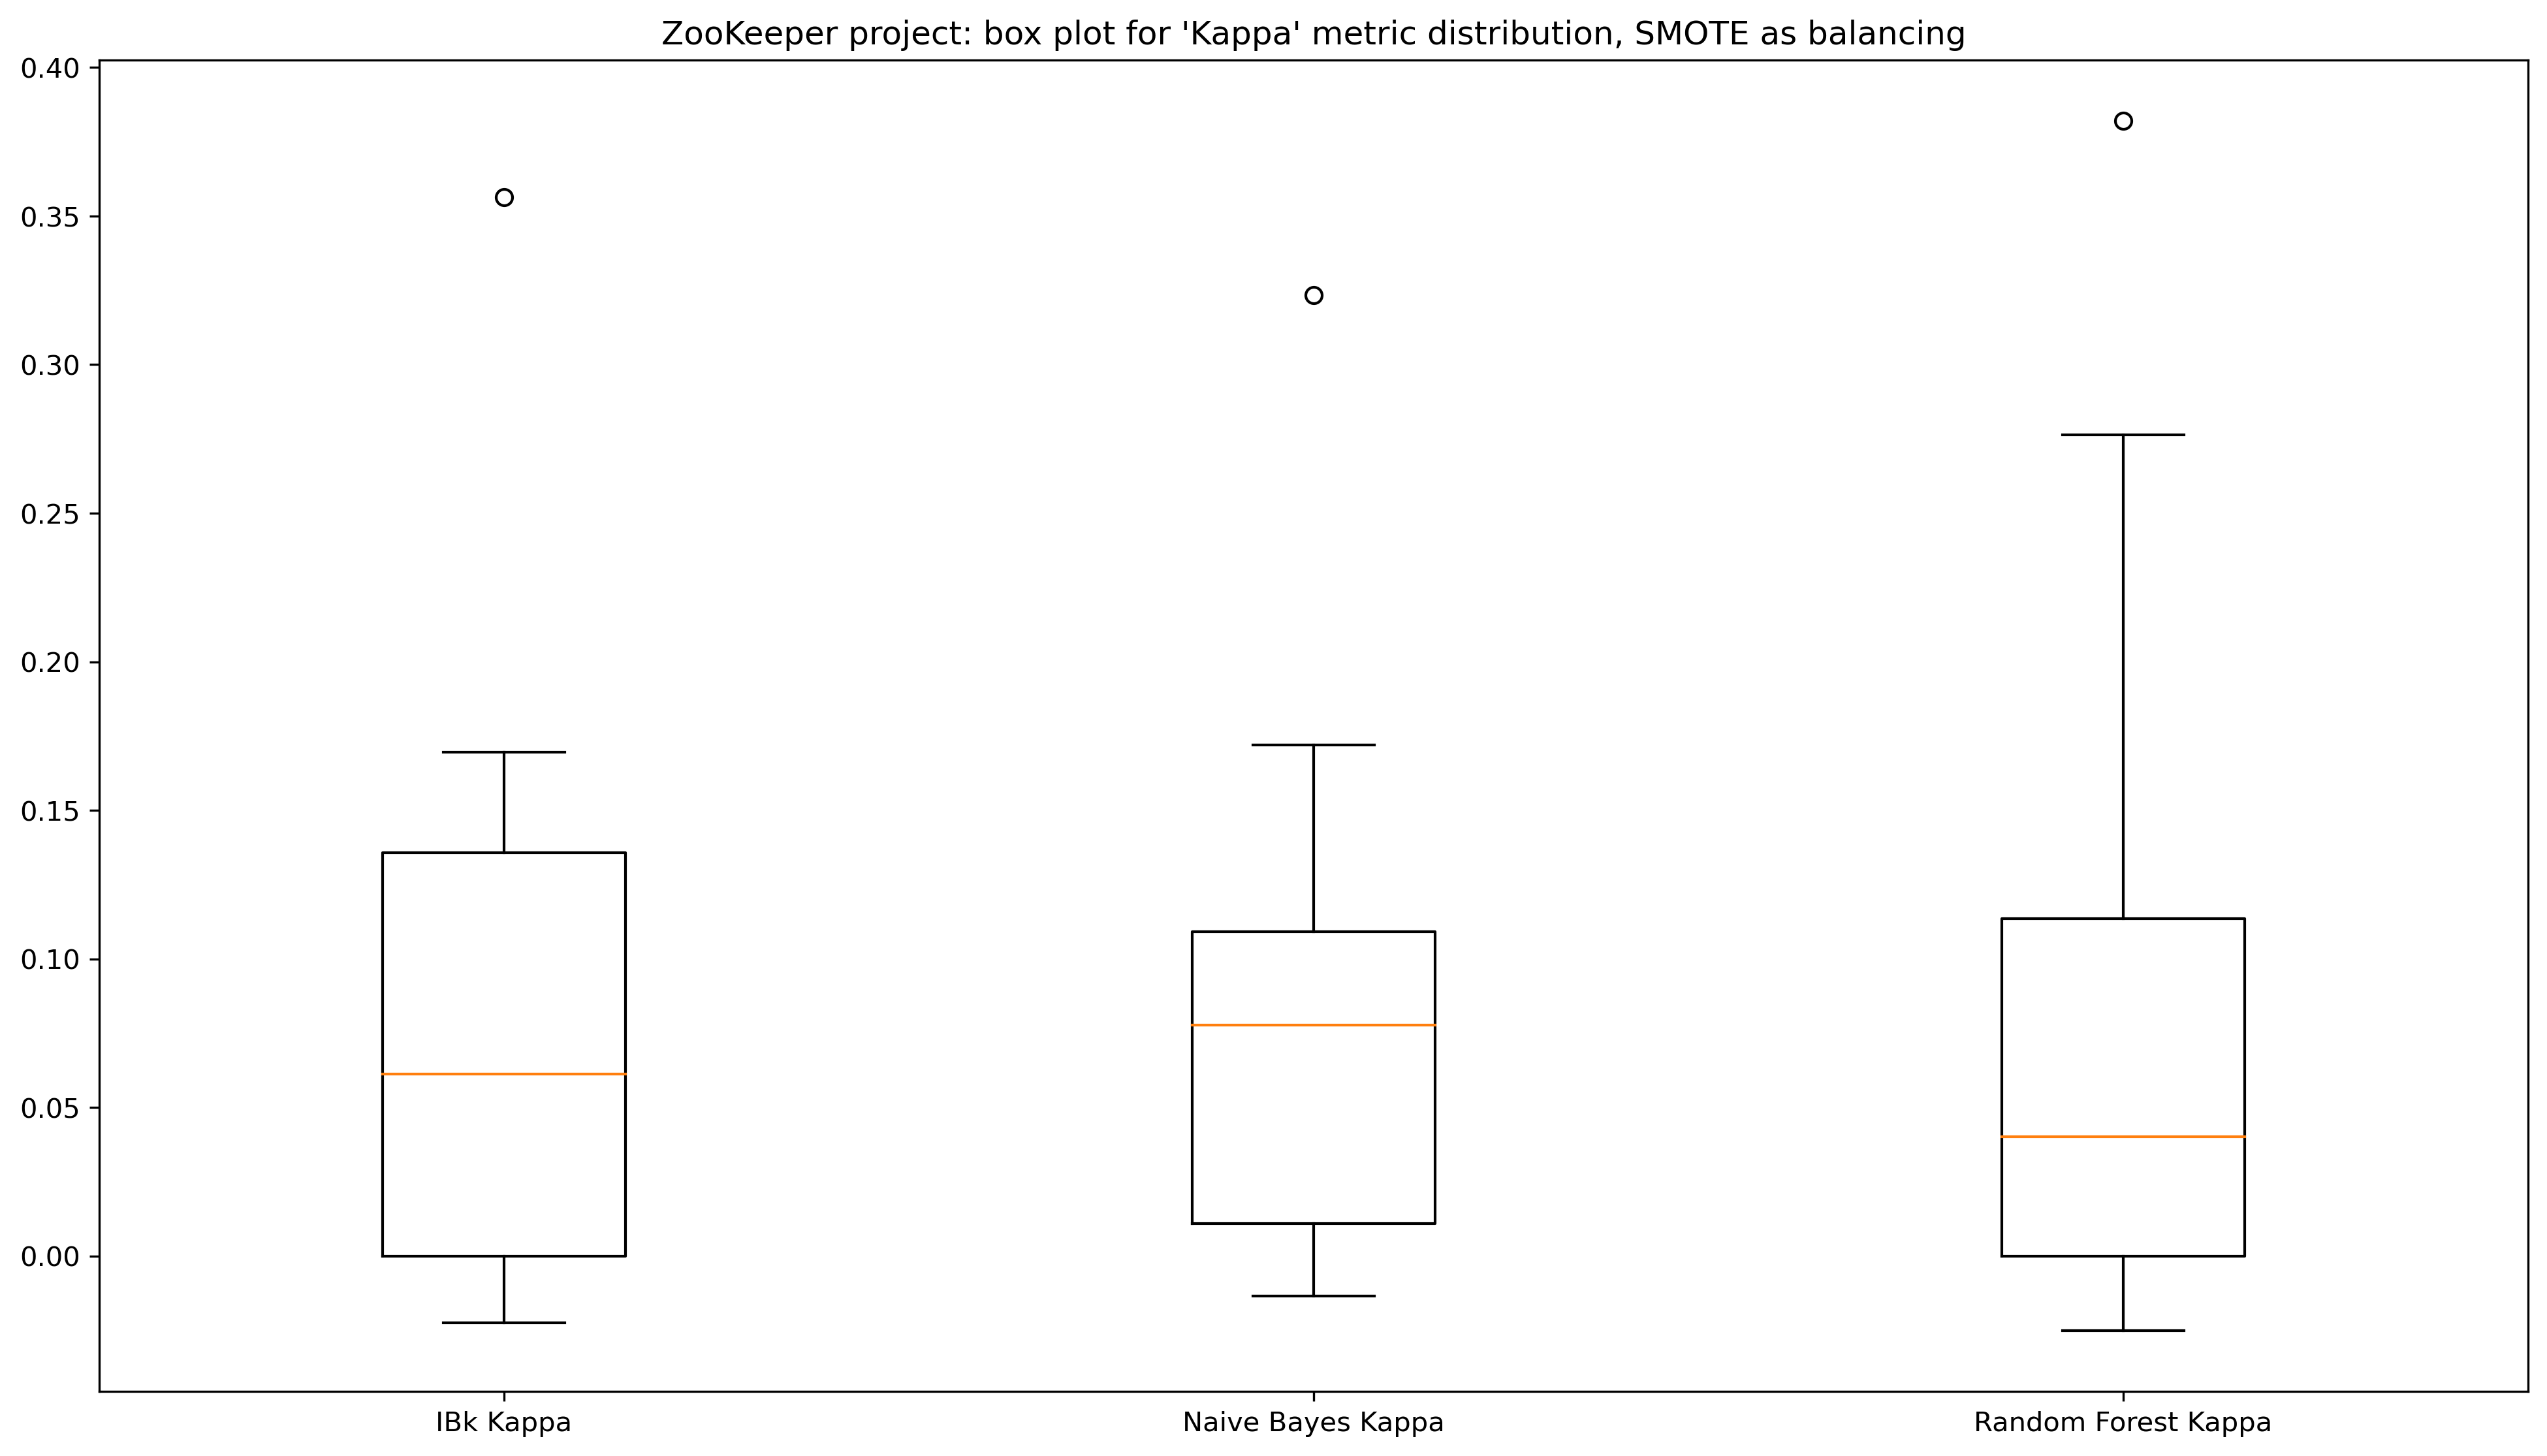
\includegraphics[scale=0.25]{images/k_bett_zk}
\end{figure}
\item La distribuzione presenta alcuni valori negativi, quindi per le relative run i classificatori si comporta peggio fi uno random, ma questo è nuovamente dovuto al dataset usato per il testing set, che presenta pochi valori positivi
\end{itemize}
\end{frame}

\begin{frame}
\section{Medie dei valori per Kappa}
\frametitle{Medie dei valori per AUC}
\begin{minipage}[t]{0.5\textwidth}%
\begin{figure}
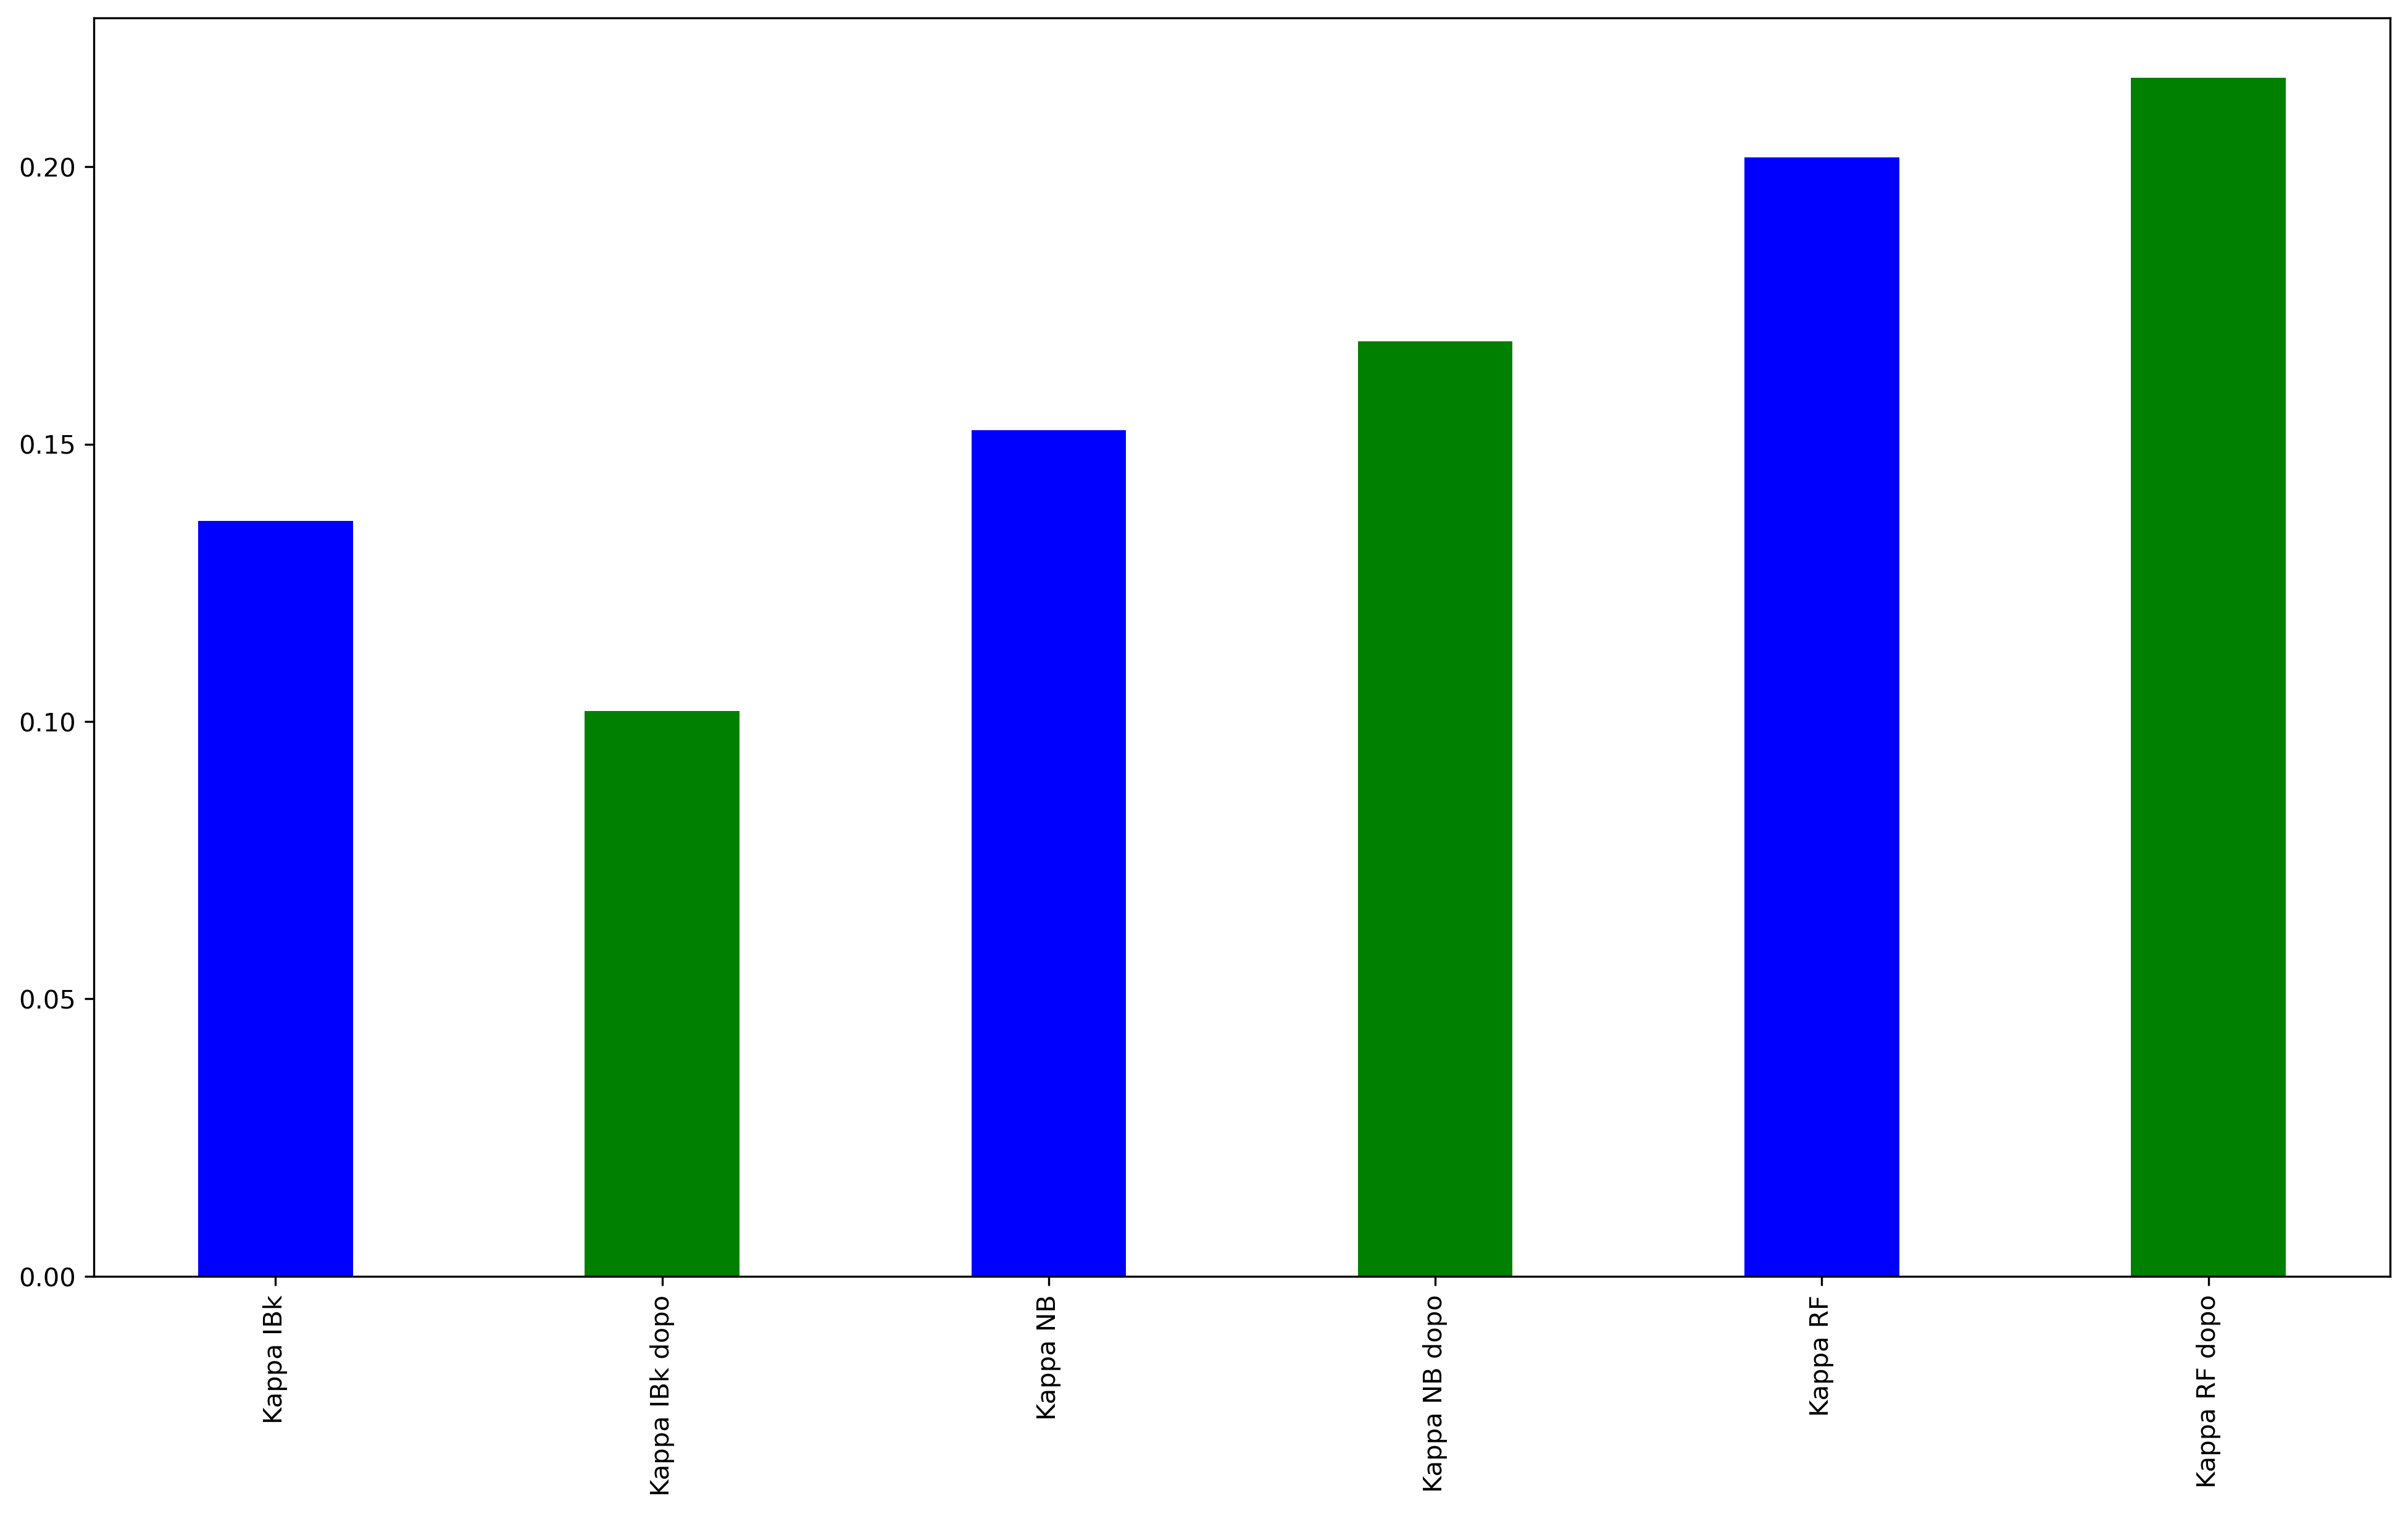
\includegraphics[scale=0.18]{images/k_bar_bk}
\caption{Confronto dei valori di Kappa per il progetto BookKeeper}
\end{figure}
\end{minipage}%
\begin{minipage}[t]{0.5\textwidth}
\begin{figure}
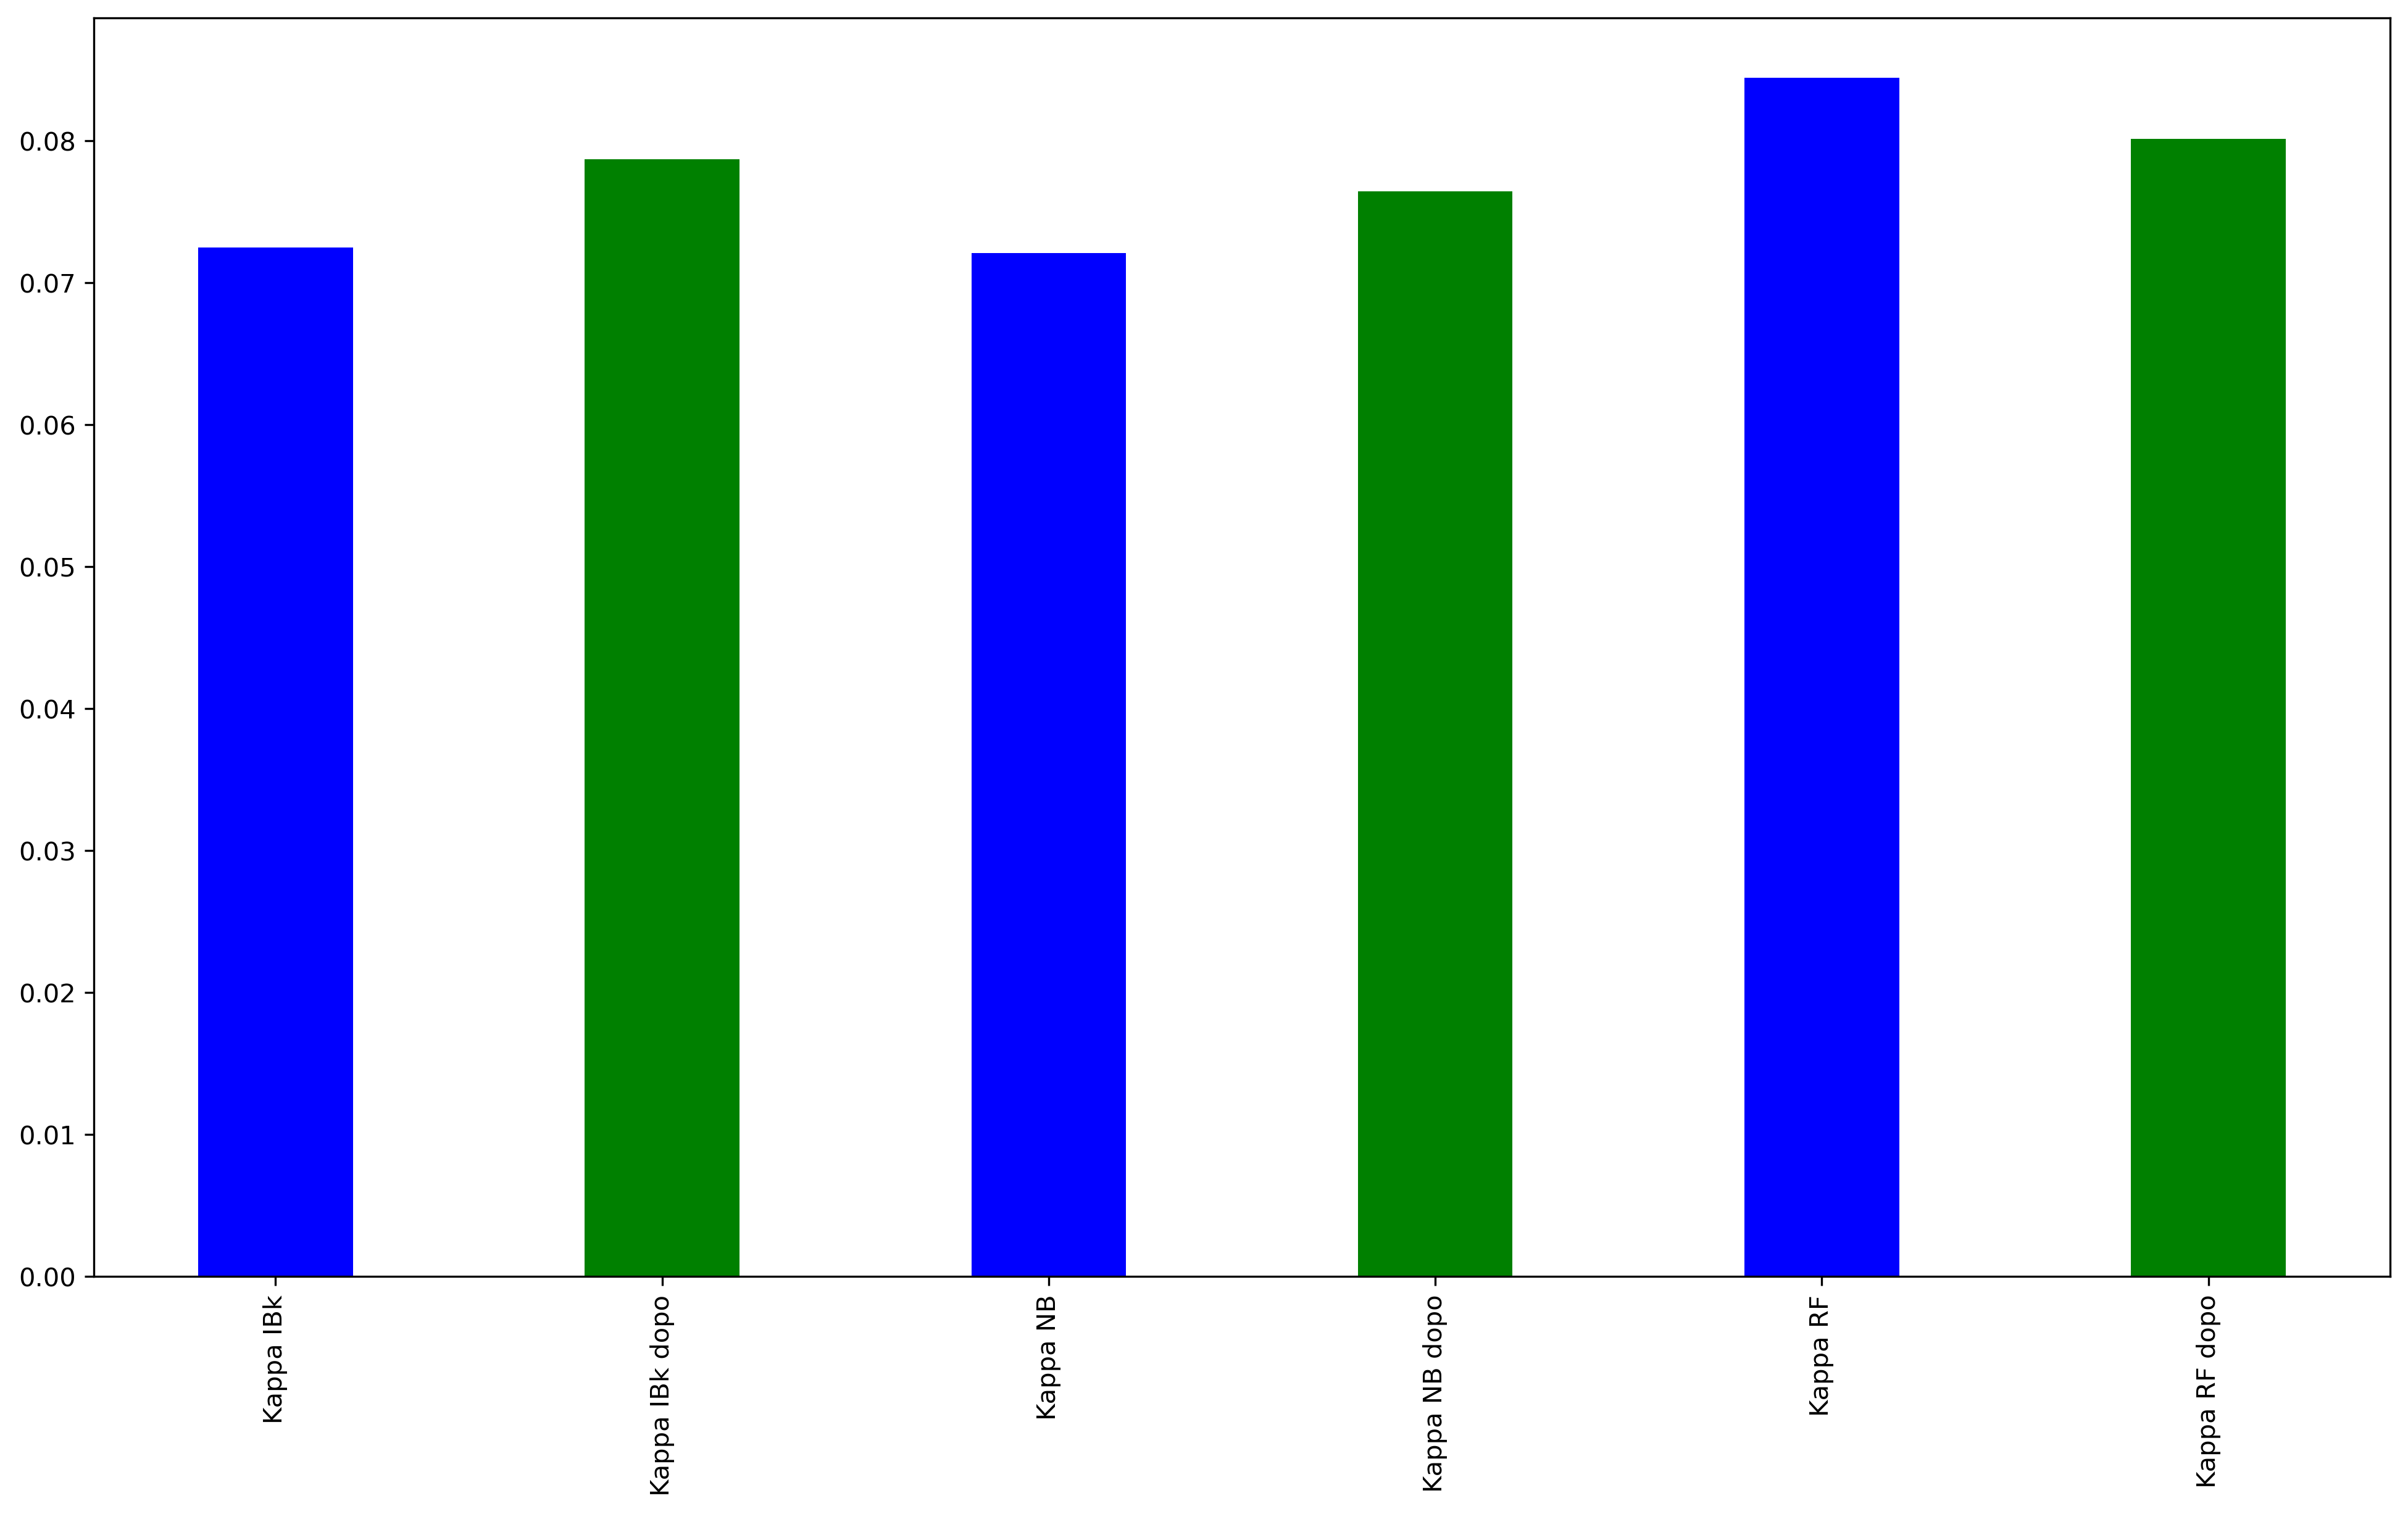
\includegraphics[scale=0.18]{images/k_bar_zk}
\caption{Confronto dei valori di Kappa per il progetto ZooKeeper}
\end{figure}
\end{minipage}
\end{frame}

\end{document}